% !TeX program = xelatex
% !Mode:: "TeX:UTF-8"
%%  本模板推荐以下方式编译: xelatex
%%     1. 文件默认的编码为 UTF-8 对于windows,请选用支持UTF-8编码的编辑器。
%%   2. 若是模板有什么问题,请及时与我们取得联系,Email:latexstudio@qq.com。
%%   3. 可以到  https://ask.latexstudio.net 提问
%%   4. 请安装 最新版本的 TeXLive 地址:
%%   http://mirrors.ctan.org/systems/texlive/Images/texlive.iso

\documentclass[12pt,a4paper]{nmmcm}
\usepackage{ctex}
\usepackage{graphicx}
\usepackage{booktabs,colortbl}
\usepackage{xcolor}
\usepackage{tikz}
\usepackage{indentfirst}
\mcmsetup{CTeX = true,
        tcn ={\xiaowuhao 2024030125260 }, problem = C,
        sheet = true, titleinsheet = false, keywordsinsheet = true,
        titlepage = true, abstract = true}
\usepackage{xurl}
\setmainfont[
    Path=fonts/TimesNewRoman/,
    UprightFont = *-Regular,
    BoldFont = *-Bold,
    ItalicFont = *-Italic,
    BoldItalicFont = *-Bold-Italic
]{TimesNewRoman}
\setmonofont[
    Path=fonts/UbuntuMono/,
    UprightFont = *-Regular,
    BoldFont = *-Bold,
    ItalicFont = *-Italic,
    BoldItalicFont = *-Bold-Italic
]{UbuntuMono}
\usepackage{lipsum}

\usepackage{paralist}
\let\itemize\compactitem
\let\enditemize\endcompactitem
\let\enumerate\compactenum
\let\endenumerate\endcompactenum
\let\description\compactdesc
\let\enddescription\endcompactdesc

\setlength\abovedisplayskip{5pt}
\setlength\belowdisplayskip{-8pt}
\setlength{\parskip}{0.1em}

\newcommand\wordc[1]{\textbf{#1}}
\renewcommand{\appendixtocname}{附\quad录}
\renewcommand{\appendices}{\hspace{-2em}{\sanhao\HEI {\bf 附~~~录}}}
\colorlet{tableheadcolor}{gray!25} % Table header colour = 25% gray
\newcommand{\headcol}{\rowcolor{tableheadcolor}}

\title{{可持续发展视角下的华北山区农作物种植策略的优化分析}}
\date{}

\usepackage[font=small,labelfont={bf,sf},tableposition=top]{caption}

% 我们团队自己的定制化操作
%%%%%%%%%%%%%%%%%%%%%%%%%%%%%%%%%%%%%%%%%%%%%%%%%%%%%%%%
\makeatletter
% 修改 section
\renewcommand\section{\@startsection{section}{1}{0pt}%
    {3.5ex plus 1ex minus .2ex}%
    {2.3ex plus .2ex}%
    {\normalfont\LARGE\bfseries}}
% 修改 subsection
\renewcommand\subsection{\@startsection{subsection}{2}{0pt}%
    {3.25ex plus 1ex minus .2ex}%
    {1.5ex plus .2ex}%
    {\normalfont\Large\bfseries}}
    % subsubsection标题的缩进
\renewcommand\subsubsection{\@startsection{subsubsection}{3}{1em}%
  {4ex plus 1ex minus .2ex}%
  {0.2ex plus .2ex}%
  {\normalfont\large\bfseries}}
\makeatother

\usepackage[backend=biber,style=gb7714-2015,gbfieldtype=true]{biblatex}
\addbibresource[location=local]{references.bib}

\usepackage{float} % 图表浮动控制
\usepackage{subcaption}
\usepackage[utf8]{inputenc}
\usepackage{pdfpages}
\usepackage{color}
\usepackage{listings}
%%%%%%%%%%%%%%%%%%%%%%%%%%%%%%%%%%%%%%%%%%%%%%%%%%%%%%%%%%%%

\begin{document}
\begin{abstract}
  

%abstract---------------
{\song\xiaosihao
\setlength{\parindent}{2em}
本文通过分析华北山区的某乡村2023年农作物种植和相关统计数据,结合未来的预期销售量、种植成本、亩产量和销售价格等多方面因素,为该乡村制定了2024至2030年的农作物种植策略。通过构建数学模型,并考虑滞销、价格波动、市场需求等不确定因素,对最优种植方案进行了分析。本研究不仅为乡村提供了一套合理的种植方案,还对未来乡村经济的可持续发展具有一定的借鉴意义。

\setlength{\parindent}{2em} 针对问题一,我们建立了一个线性规划模型,最大化每年的种植收益。模型考虑了种植面积、销售量、售价和种植成本等因素。我们通过两种情境(即作物过剩时,超出部分滞销或以半价出售)来优化种植策略。在该问题中,决策变量为每块地的种植面积,目标函数为经济收益最大化,通过求解器在各约束条件下得出最优的种植方案。该模型为乡村制定科学合理的种植计划提供了基础。

\setlength{\parindent}{2em} 针对问题二,我们进一步考虑了农作物的市场需求、售价和种植成本的年度波动。通过引入销售量、售价和成本的年度动态变化,我们扩展了线性规划模型,使其能够应对市场波动。例如考虑了小麦和玉米的销售量预计会逐年增长,而其他作物的需求在每年会有所波动等等不确定性变化。为应对这些变化,我们结合蒙特卡洛模拟进行求解,通过多次随机抽样来估计各类作物在不同市场条件下的最优种植面积分配。最终,通过统计分析,得出不同年份的种植策略与收益优化方案,为乡村应对未来市场波动提供了可靠的参考依据。

\setlength{\parindent}{2em} 针对问题三,我们考虑了农作物之间的可替代性对种植优化的影响,并基于相关性分析和线性模型,探讨了种植成本、售价和销量之间的关系。我们在问题二的基础上引入了作物之间的替代性系数,构建新的约束条件,优化了目标函数,基于回归分析结果,本文提出了一种线性模型,能够预测未来各作物的销售量,优化不同作物在不同地块上的种植面积分配。通过这一模型,乡村能够在市场条件波动较大的情况下,灵活调整作物种植面积,确保经济效益最大化,并减少因市场不确定性导致的种植风险。
}







  \begin{keywords}
    {\song\xiaosihao{ 农作物种植策略,耕地资源优化,动态规划}}
  \end{keywords}

\end{abstract}
\maketitle
\renewcommand{\contentsname}{\centerline{\sanhao\bfseries\HEI 目\quad 录}}
%\thispagestyle{empty}
%{\song\xiaosihao
% \tableofcontents
%}

\pagestyle{fancy}
\renewcommand{\headrulewidth}{0pt} % 去掉页眉的黑线
\newpage

\setcounter{page}{1}
\section{问题重述}

\subsection{问题背景}

随着乡村振兴战略的深入推进,农业作为农村经济的支柱产业,正面临着一系列新的机遇与挑战。在国家政策的大力支持下,如何有效利用有限的耕地资源,优化农作物的种植结构,提升产量和经济效益,是农村地区农业发展所必须考虑的问题。近年来,由于气候变化、农业生产资料价格波动等多重因素的影响,农村的传统农业模式正逐渐向现代化、集约化和可持续发展转型。特别是在北方山区等气候条件相对严峻的地区,因地制宜发展高效、低风险的种植策略,已成为农民增收和农村经济可持续发展的关键举措。

本文所研究的乡村位于华北山区,常年温度偏低,大部分耕地每年只能种植一季农作物。该地区的耕地资源相对分散,土地类型多样,包括平旱地、梯田、山坡地和水浇地等,适宜种植粮食作物和蔬菜。此外,随着大棚种植技术的推广,该乡村拥有普通大棚和智慧大棚,可以实现蔬菜的反季节种植。然而,如何在有限的耕地资源下,结合市场需求、种植成本和销售价格等多方面因素,制定出最优的农作物种植策略,是该乡村实现农业经济效益最大化的重要课题。通过合理的种植方案,不仅可以提高产量,减少浪费,还能够降低因市场波动和气候变化带来的种植风险。

为了实现这一目标,本文将通过建立数学模型,综合考虑该乡村现有耕地的类型、2023年农作物种植情况以及未来农作物的销售量、种植成本、亩产量和销售价格等多个因素,制定2024至2030年的最优种植策略。尤其是在粮食类作物、水稻、蔬菜、食用菌等作物的种植规划中,将充分考虑每种作物的耕作需求和市场预期,确保在最小的耕作成本下实现最大化的收益。同时,本研究还将对可能的滞销和市场波动进行风险评估,以减少种植过程中可能出现的损失。

\subsection{问题要求}

该题目要求我们为某乡村在2024至2030年期间制定最优的农作物种植策略,该乡村的耕地资源有限,主要包括1201亩露天耕地和20个大棚(16个普通大棚和4个智慧大棚)。这些耕地类型各异,包括平旱地、梯田、山坡地和水浇地,不同的耕地适宜种植不同类型的作物。此外,乡村的农作物种植还受到气候条件的限制,大多数露天耕地每年只能种植一季作物,而大棚耕地则可以种植两季作物或进行复合种植。

本文需要从以下几个角度进行问题分析与建模:
\begin{enumerate}
  \item 在2024至2030年期间,假定各种农作物的预期销售量、种植成本、亩产量和销售价格保持稳定,并且每季种植的作物当季销售。如果某种作物每季的总产量超过了其预期销售量,则有两种可能情况:第一,超过部分作物会滞销并造成浪费;第二,超过部分作物将以2023年销售价格的50\%进行降价出售。我们需要针对这两种情况,分别制定最优的种植策略,并将结果分别填入给定的Excel模板中(result1\_1.xlsx和result1\_2.xlsx)。

  \item 在实际市场中,小麦和玉米的销售量预期在未来会逐年增长,增长率介于5\%到10\%之间;其他农作物的预期销售量则可能相对于2023年有所波动,波动范围在±5\%之间。此外,气候变化等外部因素也会影响农作物的亩产量,其波动范围大约在±10\%之间。与此同时,农作物的种植成本预计将以5\%的年均增长率上涨,而蔬菜的销售价格预计每年将增长5\%,食用菌(尤其是羊肚菌)的销售价格则会逐年下降。我们需要结合这些因素,进一步建立数学模型,综合分析这些不确定性对种植策略的影响,制定更为优化的种植方案,并将结果填入result2.xlsx。

  \item 各种农作物之间的可替代性和互补性是影响农作物种植策略的重要因素之一。此外,预期销售量与销售价格、种植成本之间也存在一定的相关性。这些因素增加了农作物种植决策的复杂性,因此,我们还需要在问题2的基础上,通过对相关因素进行模拟分析,提出更具现实意义的种植策略,并与问题2的结果进行比较,验证其效果和合理性。
\end{enumerate}

本文将根据乡村的实际情况,结合问题1至问题3的要求,详细分析不同农作物的种植方案,并通过数学建模、数据分析和优化算法求解,最终为该乡村制定出最优的种植策略。在这一过程中,我们不仅要考虑到每种农作物的种植需求和市场预期,还要充分考虑滞销、价格波动等市场不确定性,以确保种植方案的科学性和可操作性。



\section{问题分析}

\subsection{问题一的分析}

针对问题一,我们需要为乡村在2024至2030年期间制定最优的农作物种植方案。农作物的种植策略优化问题实际上是一个资源分配问题,其核心在于如何合理分配有限的耕地资源,确保每种作物的种植面积既能满足市场需求,又不至于过度生产而导致滞销或降价出售。因此需要构建一个基于供需平衡的目标函数,考虑作物的亩产量、销售量以及市场需求等因素。我们可以借助线性规划或整数规划模型来求解这个资源分配问题,通过优化算法进行求解,最终得到最优的种植方案。
对于第一种情况,即超出预期销售量的部分滞销并浪费,要求设置一个约束条件,确保每种作物的种植面积不会超过其预期销售量。
对于第二种情况,超出部分降价50\%出售,我们可以允许部分作物的种植面积超过预期销售量,但需要在模型中引入价格折扣的因素,从而进一步调整目标函数,使得种植面积的增加在收益和降价之间取得平衡。


\subsection{问题二的分析}

问题二要求我们在不确定性条件下制定最优的种植策略,主要涉及销售量、产量、种植成本及市场价格的动态变化。为此,我们首先需要对销售量的增长进行预测,尤其是小麦和玉米的预期增长率,以及其他作物可能的波动。我们可以使用时间序列模型(如ARIMA)或指数平滑法进行预测,从而确定未来几年的需求变化。
种植成本和销售价格的变化也需要纳入模型,例如蔬菜价格的年均增长率和食用菌价格的下降趋势,这些动态变量将直接影响到作物的最终收益。
为了在不确定性条件下优化种植方案,我们可以采用通过蒙特卡洛模拟或鲁棒优化的方法,结合销售量、亩产量、种植成本和价格的不确定性来求解。最终给出一组最优种植方案,从而在保证收益的同时,规避因市场波动等带来的潜在风险。

\subsection{问题三的分析}

问题三要求进一步考虑作物之间的可替代性、互补性以及市场相关性。首先需要通过历史数据分析作物之间的相关性,确定哪些作物在市场上具有互补性或可替代性。作物的互补性可能使它们在同一季节同时种植能够互相提升收益,而可替代性则可能促使我们根据市场需求调整种植比例。
此外可以通过多变量回归分析或协方差矩阵量化销售量、价格和种植成本之间的相关性,分析市场上的价格波动如何影响种植成本以及最终的收益。
也可以通过采用博弈论模型来分析作物之间的竞争关系,或通过多目标优化模型在收益、成本和市场需求之间找到平衡点。从而制定出一套更为合理的种植策略,并与问题二的结果进行详细比较,以确定在多变的市场条件下如何更好地进行资源配置。


\section{模型假设}

\textbf{假设一}:农作物的市场价格保持稳定,粮食类作物价格不变,蔬菜价格每年增长5\%,食用菌价格每年下降1\%至5\%。

\textbf{假设二}:耕地资源和大棚面积在2024至2030年期间保持不变,土壤质量稳定。

\textbf{假设三}:同一地块(含大棚)不能连续重茬种植,且三年内必须种植至少一次豆类作物。

\textbf{假设四}:农作物的预期销售量基于2023年数据,且小麦、玉米销售量每年增长5\%至10\%,其他作物的销售量波动在±5\%。

\textbf{假设五}:农作物的种植成本每年按5\%的速度增长,其他投入成本稳定。

\textbf{假设六}:不同作物之间具有互补性和可替代性,这些相关性可以通过历史数据量化。


\section{符号说明}
\begin{table}[htbp]
\centering
\caption{符号说明}
\renewcommand{\arraystretch}{1.2}
\setlength{\tabcolsep}{10pt}
\begin{tabular}{p{3cm} | p{10cm}}
\hline
\hline
\textbf{符号} & \textbf{说明} \\
\hline
$S_{jk}$ & 第 $k$ 年第 $j$ 作物的期望销量 \\
$Y_{jk}$ & 第 $k$ 年第 $j$ 作物的单位面积产量 \\
$P_{jk}$ & 第 $k$ 年第 $j$ 作物的售价 \\
$C_{jk}$ & 第 $k$ 年第 $j$ 作物的单位面积成本 \\
$A^1_{ijks}$ & 第 $k$ 年第 $s$ 季度的第 $i$ 大棚上,第 $j$ 作物的种植面积 \\
$A^2_{ijks}$ & 第 $k$ 年第 $s$ 季度的第 $i$ 非大棚地块上,第 $j$ 作物的种植面积 \\
$A_{ijk}$ & 第 $k$ 年第 $i$ 地块上,第 $j$ 作物的总种植面积,定义为:\\
 & $A_{ijk} = \sum_s A^2_{ijks} + A^1_{ij(k-1)2} + A^1_{ijks}$ \\
$\text{Field Area}_i$ & 第 $i$ 地块的总面积 \\
$\text{Field Type}_i$ & 第 $i$ 地块的类型(如平旱地、梯田、水浇地) \\
$\text{Beans}$ & 豆类作物的集合 \\
$\text{Grains}_A$ & A类粮食作物的集合 \\
$\text{Grains}_B$ & B类粮食作物的集合 \\
$\text{Vege}_A$ & A类蔬菜的集合 \\
$\text{Vege}_B$ & B类蔬菜的集合 \\
$\text{Mush}$ & 食用菌的集合 \\
\hline
\hline
\end{tabular}
\end{table}




\section{模型的建立与求解}

\subsection{数据的格式化处理}
为确保数据处理的一致性和后续分析的顺利进行,我们手动对所提供数据的分隔符进行了统一。具体操作主要有三:
\begin{itemize}
  \item 将数据中的分隔符不统一问题统一转换为制表符。
  \item 将原始数据文件的编码格式由GDK转换为UTF-8编码防止出现读取乱码问题。
  \item 所有文件按照英文命名规则进行重命名,避免路径中出现中文字符。
\end{itemize}


\subsection{探索性数据分析和数据预处理}
\begin{enumerate}
  \item \textbf{查看 RAW 数据} \\
        我们首先查看了附件一和附件二中的原始数据,发现附件一数据中存在大量的缺失值(数值为$-9999$),而附件二中的数据则相对完整。
        并且我们注意到附件一中的一些非缺失数据点的的含水合物饱和度存在负值,这是明显不符合其物理意义的,也因此我们做出了这些异常数据点系仪器故障的假设。
  \item \textbf{读取数据} \\
        使用 Pandas 软件包进行数据读取,将数据存储为 DataFrame 格式,使用空值替代了缺失值的位置,方便后续的数据处理和分析。
  \item \textbf{基本可视化} \\
        我们对数据进行了基本的可视化分析,尤其关注了孔隙度和含水合物饱和度的负值情况。我们发现数据集中的孔隙度不存在数值,而在含水合物饱和度中存在负值的情况相对较多。
        \begin{figure}[H]
          \centering
          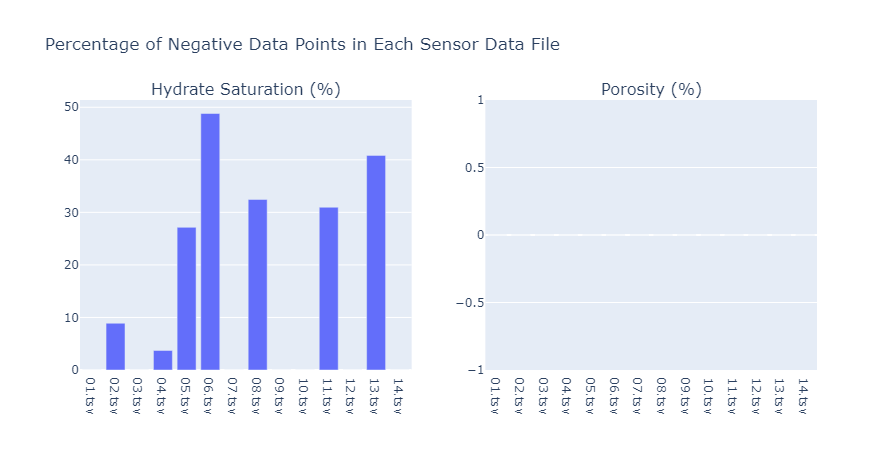
\includegraphics[width=0.7\textwidth]{figures/eda/1.png}
          \caption{含水合物饱和度(左)含孔隙度(右)在数据集中的负值情况}
        \end{figure}
  \item \textbf{数据清洗} \\
        尽管常见的Min-Max标准化方法能够有效消除负值,但同时也导致了数据的失真。标准化后的数据丧失了原有的地质学意义,放弃采用。
        因此最后对原始数据集中所有孔隙度和含水合物饱和度数值不在$[0, 1]$范围内的数据点进行了剔除。

        下图为数据清洗后的数据分布情况:
        \begin{figure}[H]
          \centering
          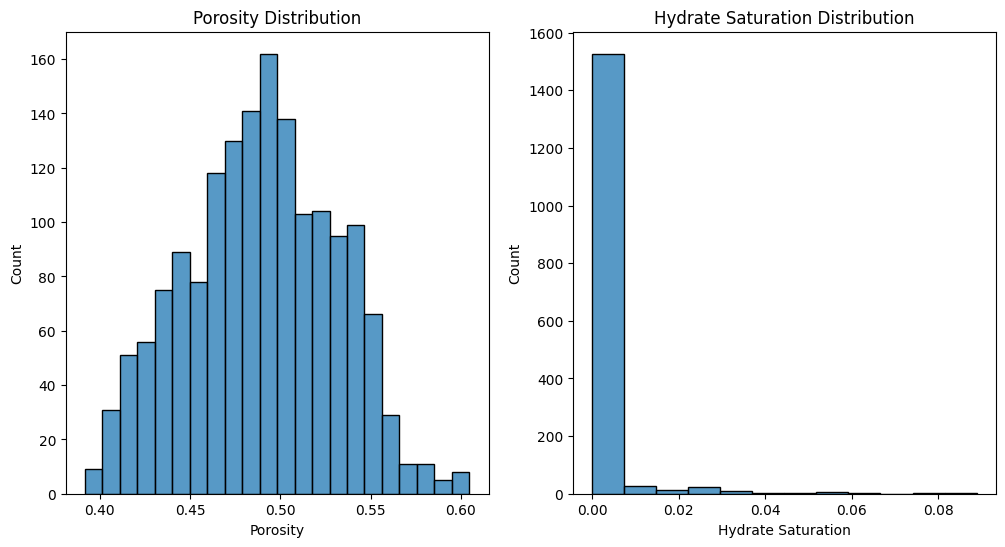
\includegraphics[width=0.7\textwidth]{figures/eda/2.png}
          \caption{孔隙度(左)和含水合物饱和度(右)在清洗后数据集中的分布情况}
        \end{figure}
\end{enumerate}

\subsection{问题1的分析和求解}
\subsubsection{问题1模型的建立}
我们需要解决的问题是根据附件中勘探井位信息,
确定天然气水合物资源分布范围,并给出详细数据和图表,在后续分析更具体的分布奠定基础。
通过对附件一和附件二中数据的观察,钻井测量数据不仅包含了深度,还包含了孔隙度和含水合物饱和度。
天然气水合物的储层参数主要包括水合物的饱和度、分布深度、分布面积、孔隙度、渗透率等,而资源量的评估更是受到了水合物饱和度、分布深度、分布面积和孔隙度的影响。
基于成藏思路的方法从本质上来讲是体积法,
体积法能反映资源的实际状态,便于指导实际开发选址,因此是体积法最常用的水合物资源量估计方法。
其数学表达如下:
\[
  Q = A \times Z \times \phi \times S \times E
\]
其中,$Q$ 为天然气水合物资源量,$A$ 为面积,$Z$ 为有效厚度,$\phi$ 为孔隙度,$S$ 为水合物饱和度,$E$ 为产气量因子。
我们假设$E$恒为$155$。而对于堪探井的每一个数据点,我们假设了它是$1$个单位面积和$0.1$单位厚度的体积内的平均情况。

因此对于任意一个数据点($x_i, y_i, z_i, \phi_i, S_i$),我们可以估算天然气水合物资源量$Q_i$:
\[
  Q_i = 1 \times 0.1 \times \phi_i \times S_i \times 155
\]


\subsubsection{问题1模型的求解}
利用预处理过后的数据,我们可以利用 Pandas、NumPy 等 Python 软件包计算每个数据点的天然气水合物资源量。

得到每个数据点的天然气水合物资源量后,我们以如下表达式计算了每一个井位中的天然气水合物资源总量:
\[
  Q_j = \sum_{i=1}^{n} Q_i, \quad \text{其中} \quad (x_i, y_i) \in \text{井位} j
\]

在得到估计的天然气水合物资源量后,我们利用 Plotly 软件包从三个角度进行了可视化分析,以帮助我们了解资源的分布情况:

\begin{enumerate}
  \item \textbf{天然气水合物资源的三维分布情况}\\
        \begin{figure}[H]
          \centering
          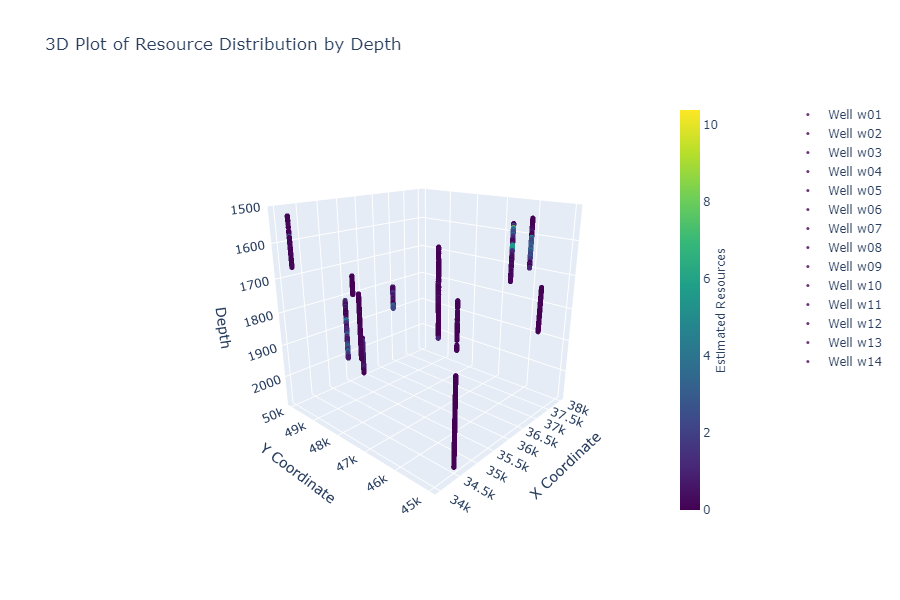
\includegraphics[width=0.9\textwidth]{figures/task1/task1-1.png}
          \caption{天然气水合物资源的三维散点图}
        \end{figure}
  \item \textbf{天然气水合物资源对于勘探井在深度上的分布情况}\\
        \begin{figure}[H]
          \centering
          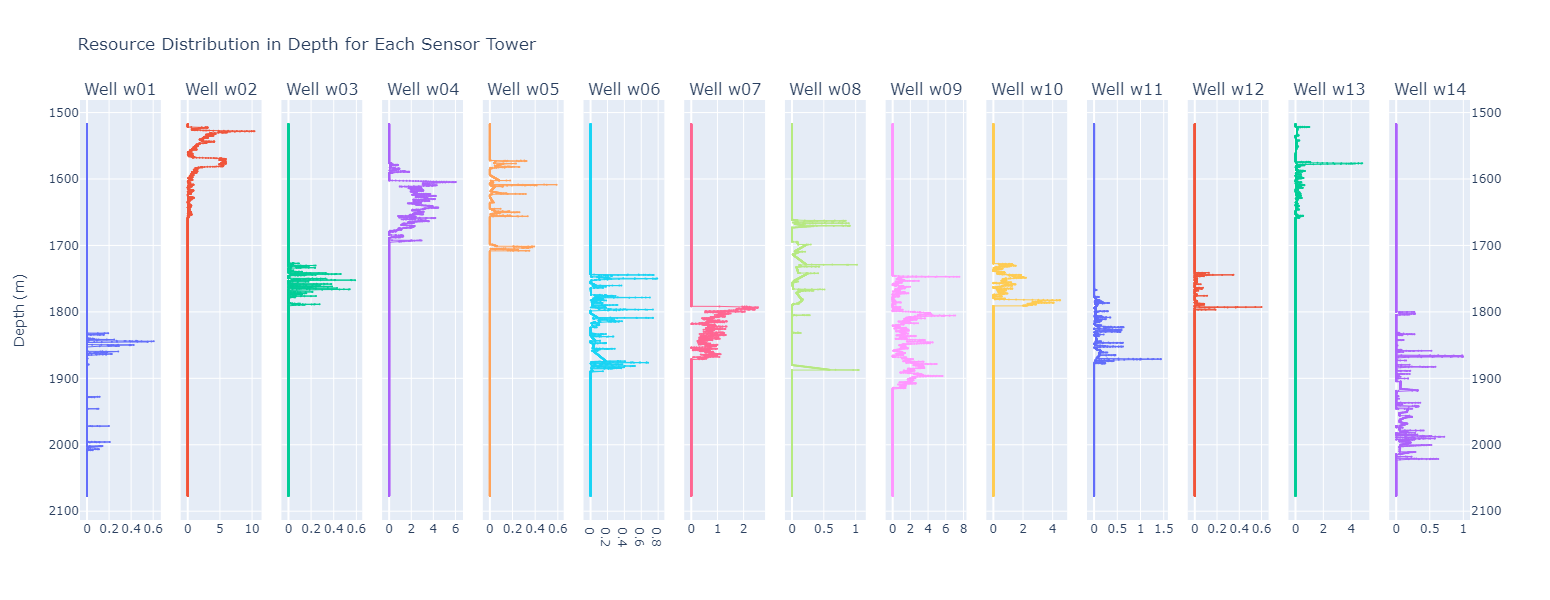
\includegraphics[width=0.99\textwidth]{figures/task1/task1-2.png}
          \caption{各井内深度与资源量的折线图}
        \end{figure}
  \item \textbf{二维平面上天然气水合物资源的分布情况} \\
        \begin{figure}[H]
          \centering
          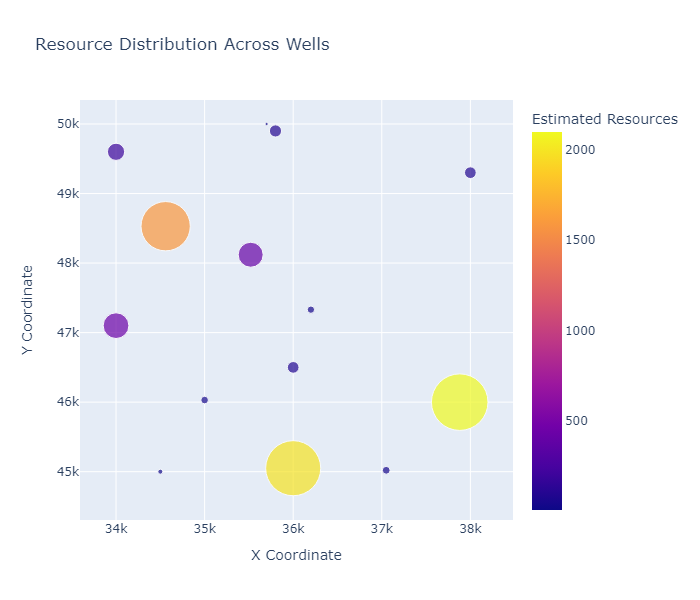
\includegraphics[width=0.7\textwidth]{figures/task1/task1-3.png}
          \caption{二维平面上天然气水合物资源的散点图}
          \label{fig:task1-3}
        \end{figure}

\end{enumerate}

\subsection{问题2模型的建立和求解}
针对问题2的模型,我们首先对三个不同指标的数据进行了预处理。对于有效厚度,我们逐一分析了14口井的数据,并剔除了不需要的点,得到每口井的有效厚度列表。随后,我们将这些数据整合,并利用正态概率分布进行拟合,得到了相应的模型。对于地层孔隙度和饱和度,我们同样采用了正态概率分布进行拟合,并获得了拟合后的图像。
进一步地,我们利用14口井的所有数据,结合井的二维坐标$(x_j,\ y_j)$和深度$z_i$构建了一个三维立体数据。在剔除了无用的点后,我们应用了三维Kriging插值模型进行随机拟合,得到了相应的立体图像。这一方法有助于我们理解勘探区域的变化规律,并为进一步的研究提供了重要参考。

\subsubsection{高斯混合模型(GMM:Gaussian Mixture Model)}
高斯混合模型是一种用于建模概率分布的统计模型。它由多个高斯分布组成,每个高斯分布代表了数据中的一个聚类。换句话说,GMM 假设数据是由多个高斯分布组成的混合物生成的,每个高斯分布对应于数据中的一个聚类或者一个潜在的生成过程。
GMM 是一种非监督学习算法,通常用于聚类分析,即将数据集划分为具有相似特征的子集。它也可以用于密度估计和异常检测。
在 GMM 中,每个高斯分布由其均值、协方差矩阵和权重参数表示。模型的目标是通过最大化似然函数或通过 EM 算法来估计这些参数,从而找到最佳的混合组合来解释数据。

\begin{enumerate}

  \item \textbf{GMM-参数} \\
        假设我们有一个观测数据集 $X = \{x_1, x_2, \ldots, x_N\}$,其中每个 $x_i$ 是一个 $D$ 维向量。
        \begin{itemize}
          \item \textbf{均值(mean):} $\boldsymbol{\mu_k}$,表示第 $k$ 个高斯分布的均值向量,$k = 1, 2, \ldots, K$。
          \item \textbf{协方差矩阵(covariance):} $\boldsymbol{\Sigma_k}$,表示第 $k$ 个高斯分布的协方差矩阵,$k = 1, 2, \ldots, K$。
          \item \textbf{混合系数(mixture coefficient):} $\boldsymbol{\pi_k}$,表示第 $k$ 个高斯分布在整个混合模型中的权重,$\sum_{k=1}^K \pi_k = 1$。
        \end{itemize}

  \item \textbf{GMM-Likelihood函数} \\
        \[
          p(X | \theta) = \prod_{i=1}^N \left( \sum_{k=1}^K \pi_k \mathcal{N}(x_i | \mu_k, \Sigma_k) \right)
        \]
        其中 \( \mathcal{N}(x | \mu, \Sigma) \) 是多维高斯分布的概率密度函数。

  \item \textbf{GMM-模型参数估计} \\
        E 步:计算每个数据点属于每个高斯分布的后验概率
        \[
          \gamma(z_{ik}) = \frac{\pi_k \mathcal{N}(x_i | \mu_k, \Sigma_k)}{\sum_{j=1}^K \pi_j \mathcal{N}(x_i | \mu_j, \Sigma_j)}
        \]

        M 步:使用后验概率重新估计参数
        \begin{align*}
          \pi_k    & = \frac{1}{N} \sum_{i=1}^N \gamma(z_{ik})                                                      \\
          \mu_k    & = \frac{\sum_{i=1}^N \gamma(z_{ik}) x_i}{\sum_{i=1}^N \gamma(z_{ik})}                          \\
          \Sigma_k & = \frac{\sum_{i=1}^N \gamma(z_{ik}) (x_i - \mu_k)(x_i - \mu_k)^T}{\sum_{i=1}^N \gamma(z_{ik})}
        \end{align*}
        重复以上 $E$ 步和 $M$ 步直到收敛,即参数不再变化或者变化很小。
\end{enumerate}

\subsubsection{基于GMM进行有效厚度和含水合物饱和度的概率分布拟合}
设函数 \(Z_j\) 表示第 \(j\) 个勘探井位的有效厚度。如果在第 \(j\) 个勘探井位中,含水化合物的起始深度为 \(d_{\text{start}, j}\) 并且终止深度为 \(d_{\text{end}, j}\),则有效厚度 \(Z_j\) 可以表示为:

\[
  Z_j = d_{\text{end}, j} - d_{\text{start}, j}
\]

接下来,对于所有的勘探井位,我们可以汇总这些数据以得到一个包含所有有效厚度的集合。这可以通过以下步骤实现:

\begin{enumerate}
  \item 从每个勘探井的数据中提取起始点和终止点。
  \item 计算每个勘探井的有效厚度 \(Z_j\)。
  \item 将所有勘探井的 \(Z_j\) 汇总到一个列表中。
\end{enumerate}

在得到数据后,使用 Python 的 SciPy 软件包中的 stats 模块,我们尝试拟合数据到各种统计模型。
通过尝试拟合不同的概率分布,我们发现使用了三个分布的高斯混合模型对数据的拟合效果最佳,达到了预期的效果。

\begin{enumerate}
  \item \textbf{有效厚度拟合曲线} \\
        \begin{figure}[H]
          \centering
          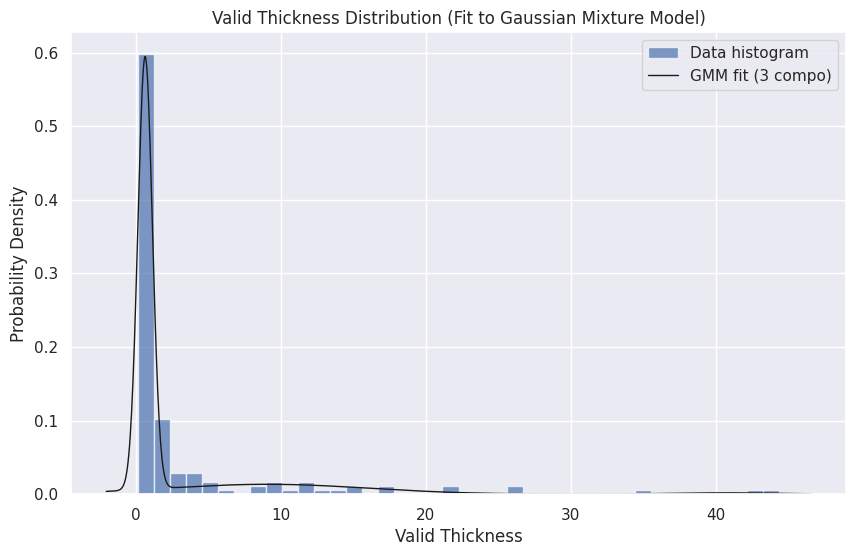
\includegraphics[width=0.8\textwidth]{figures/task2/task2-1.png}
          \caption{有效厚度的高斯混合模型}
        \end{figure}
        在这种情况下,通过调试参数,我们发现选择 3 个高斯分布来拟合数据效果最好,即模型在三个成分时达到了最佳的拟合效果,或者说能够最好地解释数据的分布特征。这通常表明有效厚度数据中存在三个明显的聚类或者生成机制。
  \item \textbf{含水合物饱和度的数据准备和预处理} \\
        将14口井的饱和度的数据放到一个tsv文件中,同时对与无效的数据以及0点进行剔除,得到一个干净的数据集,用于高斯混合模型的拟合。

  \item \textbf{含水合物饱和度的拟合曲线} \\
        \begin{figure}[H]
          \centering
          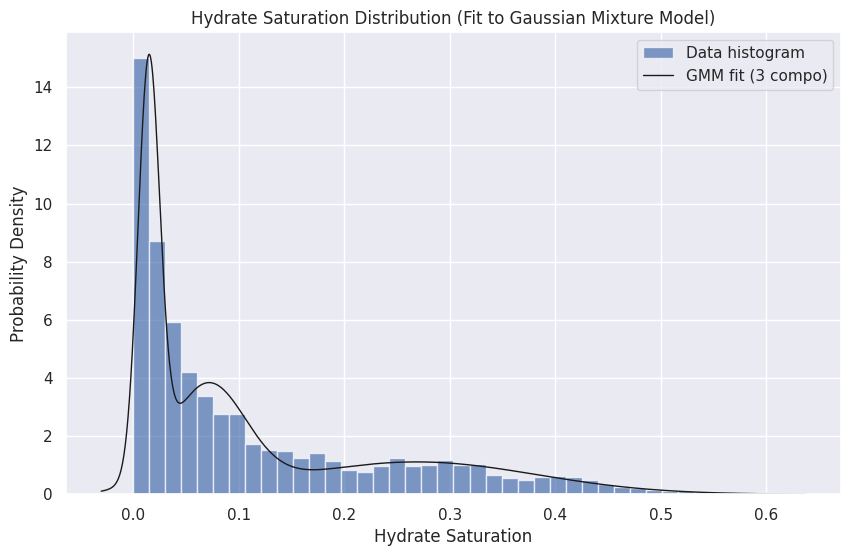
\includegraphics[width=0.8\textwidth]{figures/task2/task2-3.png}
          \caption{含水合物饱和度的高斯混合模型}
        \end{figure}




\end{enumerate}

\subsubsection{正态分布拟合}
正态分布拟合是指使用正态分布模型来拟合观测数据的过程。在统计学和机器学习中,我们经常需要对观测数据进行建模和分析,而正态分布是一种常用的分布模型,适用于很多自然现象和实验数据。
\begin{enumerate}
  \item \textbf{正态分布定义} \\
        假设我们有一个观测数据集 $X = \{x_1, x_2, \ldots, x_N\}$,我们希望用正态分布拟合这个数据集,求出其均值 $\mu$ 和方差 $\sigma^2$。
  \item \textbf{似然函数} \\
        正态分布的概率密度函数为:
        \[
          f(x | \mu, \sigma^2) = \frac{1}{\sqrt{2\pi\sigma^2}} \exp\left(-\frac{(x - \mu)^2}{2\sigma^2}\right)
        \]
        因此,数据集的似然函数为:
        \[
          L(\mu, \sigma^2 | X) = \prod_{i=1}^N f(x_i | \mu, \sigma^2)
        \]
        取对数似然函数:
        \[
          \log L(\mu, \sigma^2 | X) = \sum_{i=1}^N \log f(x_i | \mu, \sigma^2)
        \]
  \item \textbf{最大化似然函数} \\
        我们的目标是最大化对数似然函数以估计模型参数 $\mu$ 和 $\sigma^2$。这通常通过对参数求导并令导数为零来实现。

        对 $\mu$ 求导:

        \[
          \frac{\partial}{\partial \mu} \log L(\mu, \sigma^2 | X) = \sum_{i=1}^N \frac{\partial}{\partial \mu} \log f(x_i | \mu, \sigma^2)
        \]

        利用正态分布的导数性质,我们有:
        \[
          \frac{\partial}{\partial \mu} \log f(x | \mu, \sigma^2) = \frac{x - \mu}{\sigma^2}
        \]

        代入上式,并令导数为零:
        \[
          \sum_{i=1}^N \frac{x_i - \mu}{\sigma^2} = 0
        \]

        解得:
        \[
          \mu = \frac{1}{N} \sum_{i=1}^N x_i
        \]

        这是均值 $\mu$ 的最大似然估计。

        对 $\sigma^2$ 求导:

        \[
          \frac{\partial}{\partial \sigma^2} \log L(\mu, \sigma^2 | X) = \sum_{i=1}^N \frac{\partial}{\partial \sigma^2} \log f(x_i | \mu, \sigma^2)
        \]

        利用正态分布的导数性质,我们有:
        \[
          \frac{\partial}{\partial \sigma^2} \log f(x | \mu, \sigma^2) = -\frac{1}{2\sigma^2} + \frac{(x - \mu)^2}{2\sigma^4}
        \]

        代入上式,并令导数为零:
        \[
          \sum_{i=1}^N \left( -\frac{1}{2\sigma^2} + \frac{(x_i - \mu)^2}{2\sigma^4} \right) = 0
        \]

        解得:
        \[
          \sigma^2 = \frac{1}{N} \sum_{i=1}^N (x_i - \mu)^2
        \]

        这是方差 $\sigma^2$ 的最大似然估计。
\end{enumerate}

\subsubsection{基于正态分布进行孔隙度的概率分布拟合}
通过尝试拟合不同的概率分布,我们发现正态分布的拟合效果最佳,达到了预期的效果。
拟合出均值和标准差后,我们可以得到孔隙度的正态分布模型,并画出拟合曲线。
\begin{enumerate}
  \item \textbf{孔隙度拟合曲线} \\
        \begin{figure}[H]
          \centering
          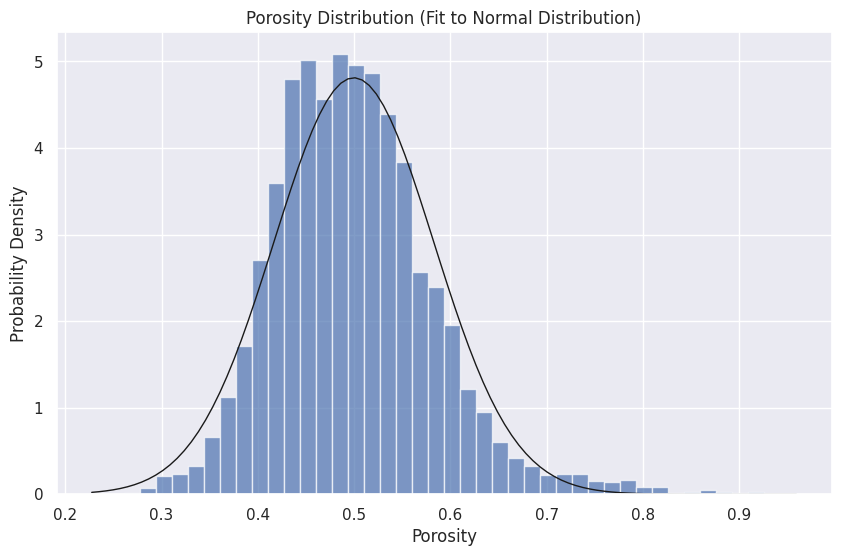
\includegraphics[scale=0.5]{figures/task2/task2-2.png}
          \caption{孔隙度的正态分布模型}
        \end{figure}
\end{enumerate}


\subsubsection{核密度估计(KDE:Kernel Density Estimation)}
核密度估计是一种非参数方法,用于估计连续随机变量的概率密度函数。它通过在每个观测数据点周围放置核函数(通常是高斯核函数),然后对所有核函数进行加权平均来估计密度。

KDE 的基本公式为:
\[
  \hat{f}_h(x) = \frac{1}{n} \sum_{i=1}^{n} K_h(x - x_i)
\]
其中:
\begin{itemize}
  \item \( \hat{f}_h(x) \) 是在点 \( x \) 处估计的密度;
  \item \( n \) 是数据点的数量;
  \item \( x_i \) 是观测数据点;
  \item \( K_h(\cdot) \) 是核函数,通常是高斯核函数,参数 \( h \) 是带宽(bandwidth),用于控制核函数的宽度。
\end{itemize}

高斯核函数 \( K_h(u) \) 的形式为:
\[
  K_h(u) = \frac{1}{\sqrt{2\pi}h} \exp\left(-\frac{u^2}{2h^2}\right)
\]

KDE 的一个关键参数是带宽 \( h \),它决定了核函数的宽度。较小的带宽会导致更细致的估计,但可能会产生过拟合;较大的带宽会导致平滑的估计,但可能会丢失一些细节。因此,选择合适的带宽对于获得良好的密度估计至关重要。

KDE 在数据可视化、密度估计、异常检测等领域都有广泛的应用。它提供了一种灵活的方法来估计数据的概率密度函数,不受特定分布形式的限制。

\subsubsection{基于KDE结果进行有效厚度变化规律分析}

我们利用 Plotly 软件包的 Contour Plot 功能,直接绘制了使用高斯内核的 KDE 方法的结果,得到了有效厚度的概率分布图。

\begin{figure}[H]
  \centering
  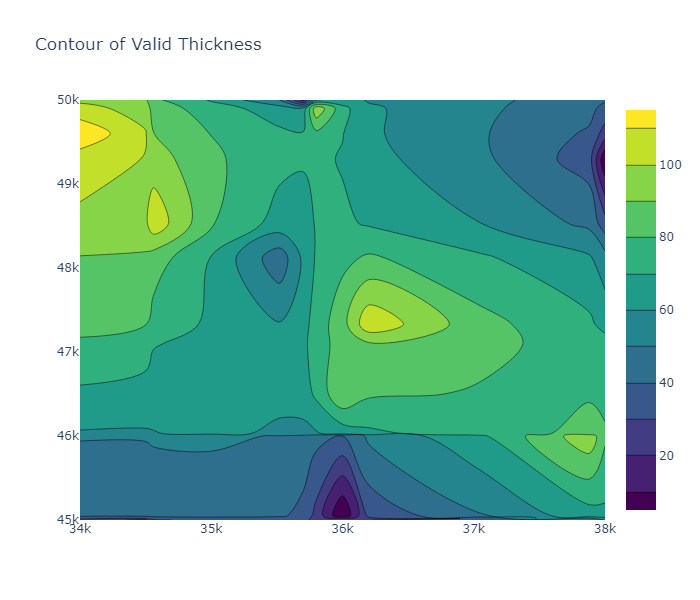
\includegraphics[width=0.7\textwidth]{figures/task2/task2-4.png}
  \caption{有效厚度的变化规律图}
  \label{fig:valid-thick-}
\end{figure}

\subsubsection{利用三维 Kriging 插值建立孔隙度、含水合物饱和度的变化模型}
Kriging 插值是一种插值和空间预测技术,常用于地理空间数据分析、地质勘探、环境科学等领域。它基于空间统计学的原理,通过对已知数据点之间的空间相关性进行建模,来预测未知位置的数值。
\begin{enumerate}
  \item \textbf{基本假设} \\
        假设我们有 $n$ 个已知的观测点 $(x_i, y_i, z_i)$,对应的观测值为 $Z(x_i, y_i, z_i)$,我们希望在未知点 $(x, y, z)$ 处估计变量值 $Z(x, y, z)$。

  \item \textbf{半方差函数的定义} \\
        假设 $h$ 是空间上两个点之间的距离,我们定义半方差函数 $\gamma(h)$ 为:

        \[
          \gamma(h) = \frac{1}{2} \text{Var}[Z(x_i, y_i, z_i) - Z(x_i+h, y_i+h, z_i+h)]
        \]

        其中,$\text{Var}[\cdot]$ 表示方差。这个公式描述了在距离 $h$ 处的两个点之间变量值的变化程度。
  \item \textbf{Kriging插值的基本公式} \\
        Kriging插值的基本公式为:

        \[
          Z(x, y, z) = \sum_{i=1}^{n} \lambda_i \cdot Z(x_i, y_i, z_i)
        \]

        其中,$\lambda_i$ 是权重,用于对已知点的观测值进行加权求和。
  \item \textbf{最小均方误差} \\
        我们希望通过最小化预测值 $Z(x, y, z)$ 与真实值 $Z(x, y, z)$ 之间的均方误差来确定权重 $\lambda_i$。
  \item \textbf{最小化均方误差的优化问题} \\
        定义误差 $e(x, y, z) = Z(x, y, z) - \sum_{i=1}^{n} \lambda_i \cdot Z(x_i, y_i, z_i)$,则我们的目标是最小化误差的平方和:

        \[
          \min_{\lambda_i} \sum_{i=1}^{n} e^2(x, y, z)
        \]
\end{enumerate}
对于孔隙度和 含水合物饱和度,我们分别构建了三维空间的 Kriging 插值模型,以便于对其进行空间预测。
经过参数的调整,我们选定 “hole-effect” 为我们的变异函数,其数学表达为:
\[
  \gamma(h) = \sigma^2 \left(1 - \exp\left(-\frac{h}{a}\right)\right)
\]
其中,$\sigma^2$ 为方差,$a$ 为相关长度。


\subsubsection{三维Kriging插值模型的求解}

利用 Python 中的 PyKrige 库,我们能够便捷地执行三维 Kriging 插值。该过程涉及将孔隙度和水合物饱和度数据输入到 Kriging 插值模型中,以生成详尽的插值结果。

鉴于涉及的数据点众多,导致 Kriging 插值计算相对耗时。为了优化计算效率,我们采取了随机抽样策略,选取了30\%的数据点进行初步的插值分析。

在模型拟合完成后,我们设定了一个分辨率为 \((60, 60, 6)\) 米的三维网格,覆盖整个勘探区域,用于进行系统的插值计算。通过应用已拟合的模型,我们在这一网格上进行了详细的插值操作,最终得到了区域内孔隙度和水合物饱和度的三维分布图,为进一步的地质评估和资源开发提供了科学依据。

\begin{enumerate}
  \item \textbf{孔隙度的 Kriging 插值结果} \\
        如图所示,孔隙度的Kriging插值结果显示了数据的空间分布与变化,插值结果的颜色渐变表明了孔隙度的变化。Kriging预测误方差图展示了预测误差较小,说明模型对数据的拟合比较精确。
        \begin{figure}[H]
          \centering
          % 第一行
          \begin{subfigure}[b]{0.3\textwidth}
            \centering
            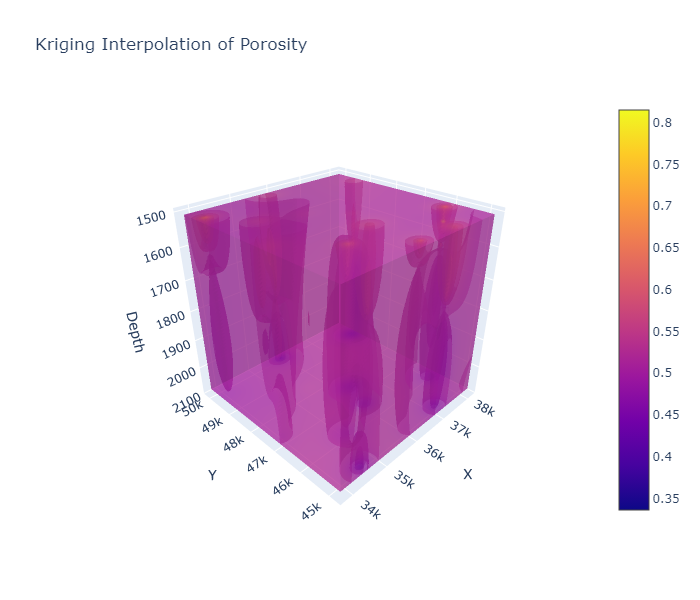
\includegraphics[width=\textwidth]{figures/task2/task2-5-1.png}
            \caption{Kriging插值结果}
            \label{fig:porosity-Kriging-3d}
          \end{subfigure}
          \hfill
          \begin{subfigure}[b]{0.3\textwidth}
            \centering
            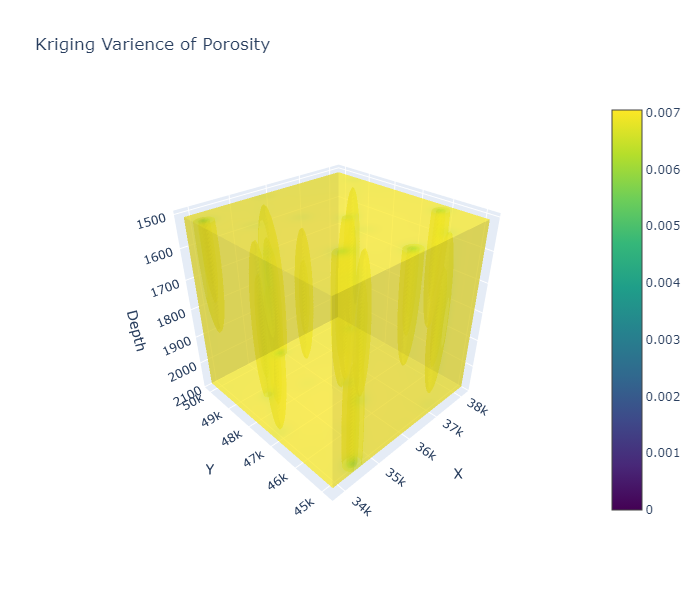
\includegraphics[width=\textwidth]{figures/task2/task2-5-2.png}
            \caption{Kriging预测误方差图}
            \label{fig:porosity-error-Kriging-3d}
          \end{subfigure}
          \hfill
          \begin{subfigure}[b]{0.3\textwidth}
            \centering
            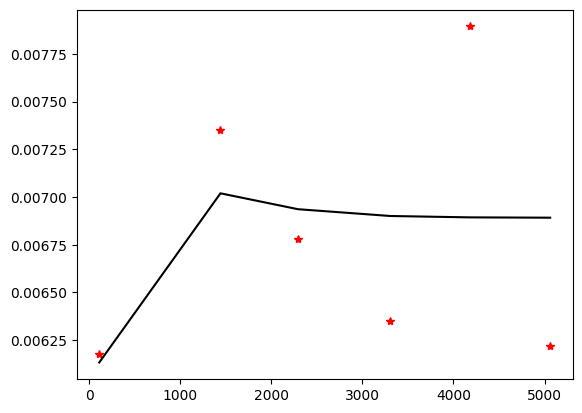
\includegraphics[width=\textwidth]{figures/task2/task2-5-3.png}
            \caption{实验半方差图结果}
            \label{fig:KrigingSemivariogram1}
          \end{subfigure}
        \end{figure}

  \item \textbf{含水合物饱和度的 Kriging 插值结果} \\
        含水合物饱和度的插值结果同样展示了空间分布特征,颜色的变化反映了饱和度的变化。预测误方差图表明模型的预测都较为准确。
        \begin{figure}[H]
          % 第二行
          \begin{subfigure}[b]{0.3\textwidth}
            \centering
            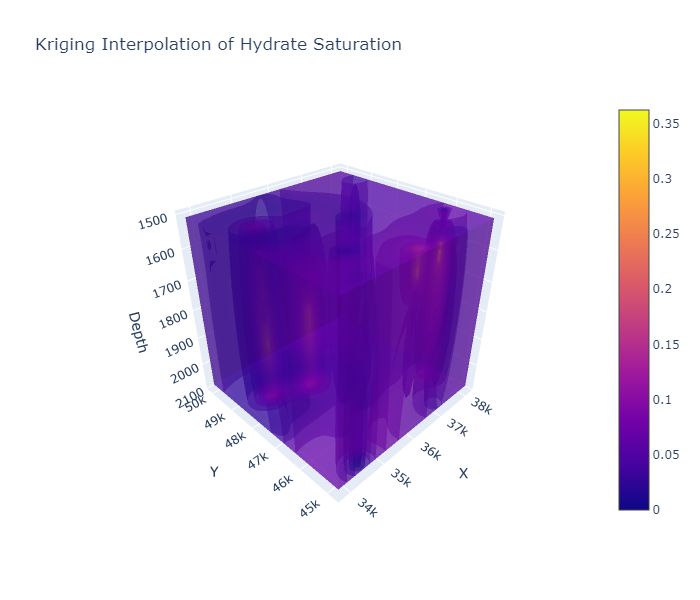
\includegraphics[width=\textwidth]{figures/task2/task2-6-1.png}
            \caption{Kriging插值结果}
            \label{fig:water-saturation-Kriging-3d}
          \end{subfigure}
          \hfill
          \begin{subfigure}[b]{0.3\textwidth}
            \centering
            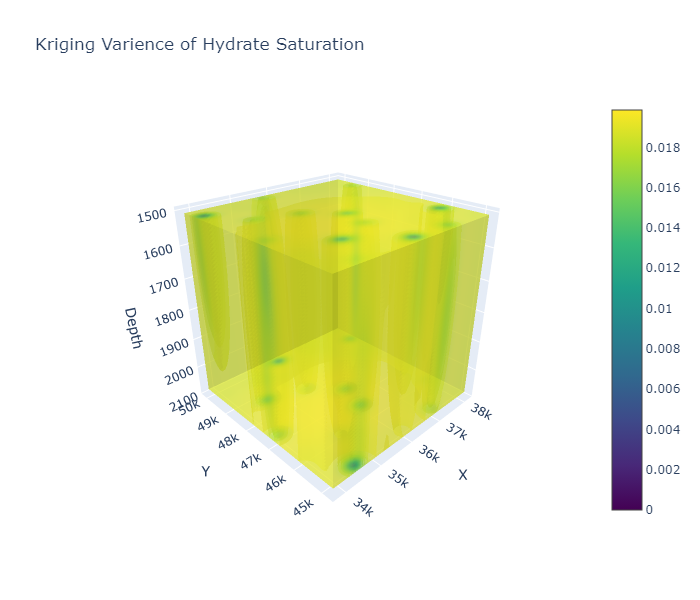
\includegraphics[width=\textwidth]{figures/task2/task2-6-2.png}
            \caption{Kriging预测误方差图}
            \label{fig:water-saturation-error-Kriging-3d}
          \end{subfigure}
          \hfill
          \begin{subfigure}[b]{0.3\textwidth}
            \centering
            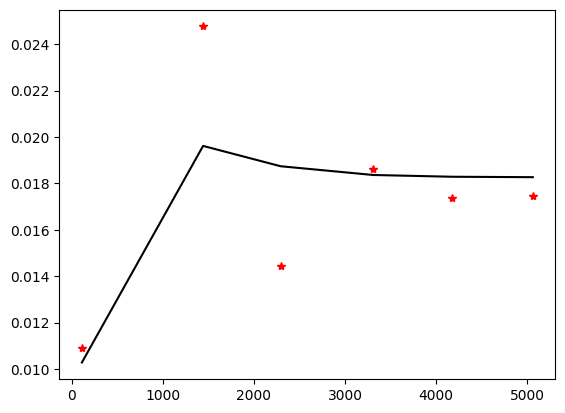
\includegraphics[width=\textwidth]{figures/task2/task2-6-3.png}
            \caption{实验半方差图结果}
            \label{fig:KrigingSemivariogram2}
          \end{subfigure}
        \end{figure}
\end{enumerate}


\subsection{问题3模型的建立和求解}

\subsubsection{资源量的概率分布模型的建立}
对于资源量的概率分布估计,我们沿用了问题2中的二维 KDE 方法,通过核密度估计来估计资源量的概率分布,并且依然采用高斯内核。

因此 KDE 计算表达式为:
\[
  f(x, y) = \frac{1}{Q_k} \sum_{i=1}^{Q_k} \frac{1}{2\pi h^2} \exp \left( -\frac{(x-x_i)^2 + (y-y_i)^2}{2h^2} \right)
\]

\subsubsection{资源量的概率分布模型的求解}
我们利用 Plotly 软件包的 Contour Plot 功能,直接绘制了使用高斯内核的 KDE 方法的结果,得到了资源量的概率分布图。

\begin{figure}[H]
  \centering
  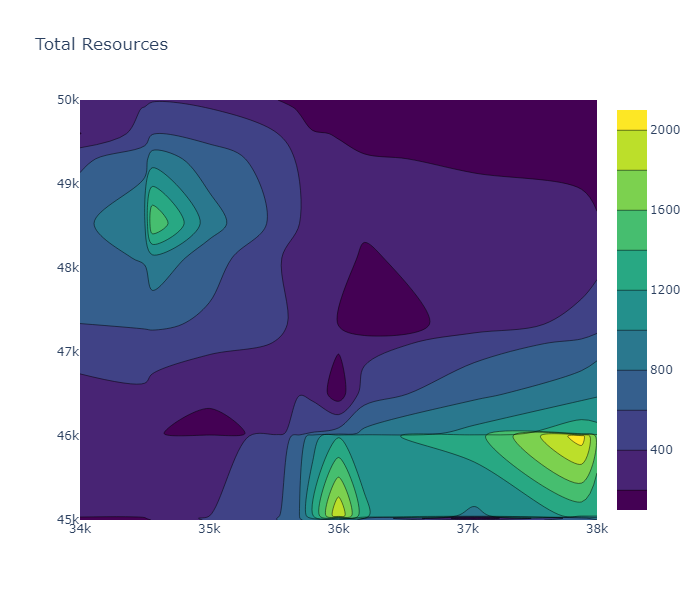
\includegraphics[width=0.45\textwidth]{figures/task3/task3-1.png}
  \caption{资源量的概率分布图}
\end{figure}

可以看到其和问题1中的图 \ref{fig:task1-3} 有较为明显的联系,这也说明了我们的模型是基本合理的。

\subsubsection{勘探区域内资源总量估计模型的建立}
而对于勘探区域内资源总量的估计,我们可以直接利用问题2中得到的孔隙度和饱和度的 Kringing 插值结果,估算空间内每个位置点的资源量,所有求和即可得到总资源量的概率分布估计。

对于这个建模我们可以得到表达式:
\begin{align*}
  Q_k & = A \times Z \times \phi \times S \times E         \\
      & = 1 \times 0.1 \times \phi_k \times S_k \times 155
\end{align*}


\[
  Q_{\text{total}} = \sum_{k=1}^{n} Q_k
\]


\subsection{问题4模型的建立和求解}
\subsubsection{二维 Kriging 插值模型的建立}
二维 Kriging 插值是一种高级的地统计学方法,用于预测空间数据的分布。在本研究中,我们使用普通Kriging插值(Ordinary Kriging)来估计未知位置的资源量,基于已知井点的资源数据。

\begin{enumerate}
  \item \textbf{数据准备和预处理} \\
        首先,我们从已有的井点数据中提取坐标 $(x_i, y_i)$ 和对应的资源量 $z_i$。这些数据点作为Kriging插值的输入,用于构建空间连续性模型。

  \item \textbf{普通Kriging插值} \\
        普通Kriging插值的基本公式可以表示为:
        \[
          Z(x) = \mu + \sum_{i=1}^n \lambda_i (Z(x_i) - \mu)
        \]
        其中,$Z(x)$ 是在位置 $x$ 的预测值,$\mu$ 是未知常数(通常是全局均值),$Z(x_i)$ 是已知数据点的值,$\lambda_i$ 是权重系数,$n$ 是用于预测的已知数据点的数量。

  \item \textbf{变异函数和模型参数} \\
        在Kriging方法中,变异函数(semivariogram)是描述空间数据点之间关系的关键。在本研究中,我们选择球形变异函数模型,其表达式为:
        \[
          \gamma(h) =
          \begin{cases}
            C_0 + C \left( \frac{3h}{2a} - \frac{h^3}{2a^3} \right) & \text{if } h \leq a \\
            C_0 + C                                                 & \text{if } h > a
          \end{cases}
        \]
        其中,$h$ 是空间距离,$C_0$ 是块金效应(nugget effect),$C$ 是基台值(sill),$a$ 是变程(range),即空间相关性的最大距离。

  \item \textbf{权重系数的确定} \\
        权重系数 $\lambda_i$ 通过解决Kriging方程来确定,确保预测误差最小化。Kriging方程可以表示为:
        \[
          \sum_{j=1}^n \lambda_j \gamma(x_i, x_j) + \mu = \gamma(x_i, x)
        \]
        对于所有 $i = 1, 2, \ldots, n$。此外,为了保证无偏估计,权重的和应该满足:
        \[
          \sum_{i=1}^n \lambda_i = 1
        \]

  \item \textbf{插值和预测} \\
        最后,使用解得的权重系数 $\lambda_i$ 和模型参数,我们可以计算任意位置 $x$ 的资源量预测值 $Z(x)$。这一过程涉及到在整个研究区域内创建一个平面网格,并在每个网格点上应用上述Kriging公式进行资源量预测。
\end{enumerate}

\pagebreak

\subsubsection{二维 Kriging 插值模型的求解}

\begin{enumerate}
  \item \textbf{实验半方差图结果分析} \\
        % Insert pics
        \begin{figure}[H]
          \centering
          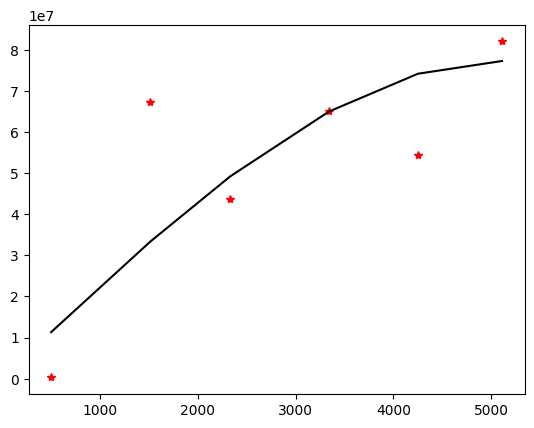
\includegraphics[width=0.3\textwidth]{figures/task4/task4-1.png}
          \caption{实验半方差图结果}
          \label{fig:KrigingSemivariogram}
        \end{figure}
        如图 \ref{fig:KrigingSemivariogram} 所示,实验半方差图显示了理论模型(黑色曲线)与实际观测数据点(红色星号)的对比。主要观察结果包括:
        \begin{itemize}
          \item 实际数据点大体上遵循理论模型的趋势,表明所选的球形变异函数模型是合适的。
          \item 在较小的空间距离 \( h \) 上,数据点与理论曲线较为接近,说明在小范围内,空间自相关性较强。
          \item 随着 \( h \) 的增加,实际数据点的分布开始波动,可能反映了在较大距离上空间自相关性的减弱。
        \end{itemize}

  \item \textbf{预测误方差与插值结果分析} \\
        \begin{figure}[H]
          \centering
          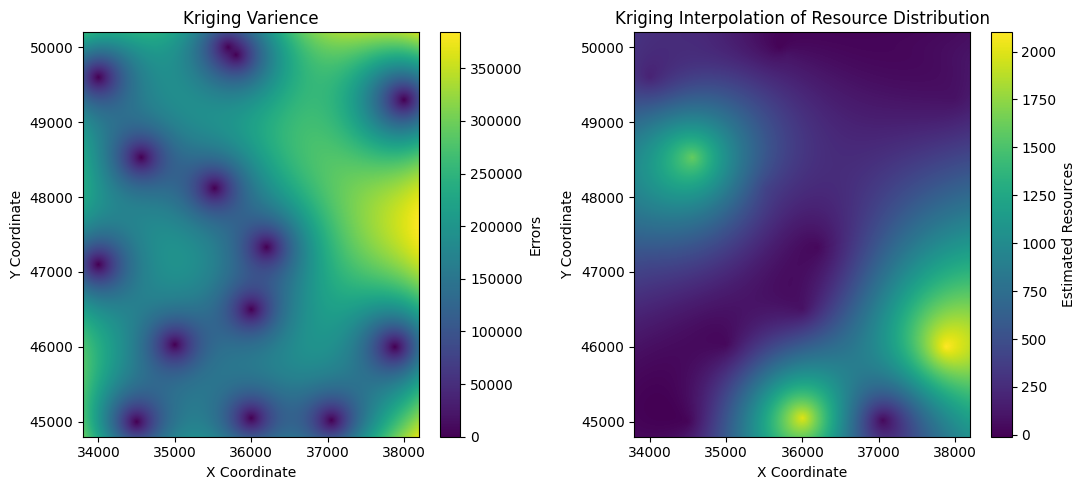
\includegraphics[width=0.8\textwidth]{figures/task4/task4-2.png}
          \caption{预测误方差(左)和 插值结果(右)}
          \label{fig:KrigingInterpolation}
        \end{figure}
        第二张图片(图 \ref{fig:KrigingInterpolation})展示了 Kriging 预测的方差(左图)和资源量的插值结果(右图)。分析如下:
        \begin{itemize}
          \item \textbf{预测误方差图(左图)}:
                \begin{itemize}
                  \item 显示了各个位置的预测误差大小,颜色越亮(趋向黄色)表示预测的不确定性越大。
                  \item 在已知数据点附近,预测误差较小,显示模型在数据点附近具有较高的信度。
                  \item 数据点间的区域预测误差增大,反映了这些区域内插值的不确定性较高。
                \end{itemize}
          \item \textbf{资源量插值结果图(右图)}:
                \begin{itemize}
                  \item 此图显示了整个区域的资源量预测分布。颜色越亮(趋向黄色)表示预测的资源量越高。
                  \item 资源量的高值区主要集中在某些特定区域,可能与原始数据点的分布和地质特性有关。
                  \item 插值结果显示了资源分布的空间变异性,有助于理解资源在研究区域内的分布特征。
                \end{itemize}
        \end{itemize}

        我们还利用二维 Kriging 插值的结果再次估计勘探区域的资源总量,即
        \[
          Q_{\text{total}} = \sum_{k=1}^{n} Q_k
        \]。
        最终的到 $50355145428.42452$ 的结果,这与问题三中利用孔隙度和饱和度的三维 Kringing 插值结果求出的资源总量 $44417499906.32$ 误差仅约为 10\%,间接验证了模型的准确性。

\end{enumerate}



\subsubsection{粒子群优化算法的数学模型}
粒子群优化(PSO)是一种基于群体的优化技术,模拟鸟群的社会行为来寻找问题的最优解。每个粒子代表潜在的解决方案,在解空间中按照简单的数学规则移动。

\begin{enumerate}
  \item \textbf{粒子的表示} \\
        在PSO中,粒子$i$在$d$维搜索空间中的位置表示为$\mathbf{x}_i = (x_{i1}, x_{i2}, \ldots, x_{id})$,速度表示为$\mathbf{v}_i = (v_{i1}, v_{i2}, \ldots, v_{id})$。每个粒子还维护一个个人最优位置$\mathbf{p}_{\text{best},i}$,即该粒子历史上遇到的最优位置。

  \item \textbf{速度和位置更新} \\
        粒子的速度和位置通过以下公式更新:
        \[
          \mathbf{v}_i^{(t+1)} = w \mathbf{v}_i^{(t)} + c_1 r_1 (\mathbf{p}_{\text{best},i} - \mathbf{x}_i^{(t)}) + c_2 r_2 (\mathbf{g}_{\text{best}} - \mathbf{x}_i^{(t)})
        \]
        \[
          \mathbf{x}_i^{(t+1)} = \mathbf{x}_i^{(t)} + \mathbf{v}_i^{(t+1)}
        \]
        其中,$w$是惯性权重,控制粒子速度的保留程度;$c_1$和$c_2$是学习因子,通常称为认知和社会参数;$r_1$和$r_2$是[0,1]区间内的随机数,代表随机性;$\mathbf{g}_{\text{best}}$是全局最优位置,即所有粒子历史上遇到的最优位置。

  \item \textbf{参数选择} \\
        惯性权重$w$通常设置为0.7至0.9之间,有助于控制搜索的全局和局部探索能力。学习因子$c_1$和$c_2$通常设置为相同的值,比如1.5,这样可以平衡个体经验和群体经验的影响。

  \item \textbf{初始化和迭代过程} \\
        每个粒子的初始位置和速度通常是随机生成的。在每次迭代中,根据上述规则更新所有粒子的速度和位置。同时,更新每个粒子的个人最优位置以及全局最优位置。迭代继续进行,直到满足最大迭代次数或其他终止条件。

  \item \textbf{目标函数和优化目标} \\
        PSO目标是找到使目标函数$J(x)$最大化的解$\mathbf{x}$。在本文中,目标函数是最大化新井位置的预测资源总量和最小化井点间的最短距离的负值。
\end{enumerate}


\subsubsection{基于 Kriging 插值的优化模型建立}

在 Kriging 插值的求解结果和粒子群优化算法的基础上,我们进一步建立了一个优化模型,旨在确定新井的最佳位置,以最大化资源的总探测量和井点之间的距离。模型的目标函数综合考虑了新井之间以及新旧井之间的最小距离和新井位置的预测资源总量。

\begin{enumerate}
  \item \textbf{目标函数定义} \\
        设计目标函数如下,用于评估新井布置的质量:
        \[
          J(x) = -\left(\min(\text{dist}(x_i, x_j)) + \sum_{k=1}^{n} Z(x_k, y_k)\right)
        \]
        其中,$n$ 为新井的数量,$x = \{(x_1, y_1), (x_2, y_2), \ldots, (x_{n}, y_{n})\}$ 表示新井的位置,$\text{dist}(x_i, x_j)$ 表示所有井点(包括现有和新井)之间的欧氏距离矩阵,$Z(x_k, y_k)$ 是在位置 $(x_k, y_k)$ 的预测资源量,通过 Kriging 插值得到。

  \item \textbf{优化算法选择} \\
        我们采用粒子群优化(PSO)算法来解决这一多目标优化问题。PSO 是一种基于群体的随机优化技术,通过模拟鸟群的社会行为来搜索最优解。在本问题中,每个粒子代表一组潜在的新井位置,粒子通过迭代更新其位置,以寻找使目标函数最大化的解。

  \item \textbf{粒子群优化参数设置} \\
        在 PSO 算法中,我们设置了如下参数:个体学习因子$c_1$、社会学习因子$c_2$和惯性权重$w$。这些参数控制粒子更新其速度和位置的方式,其中$c_1$和$c_2$通常设置为1.5,$w$设置为0.7。

  \item \textbf{约束条件和边界} \\
        新井的位置受到现有井位置的范围约束,即每个新井的坐标$(x, y)$必须在现有井的最小和最大坐标加上了 150 m 扩展的范围内。这确保了新井的位置在合理的探测区域内。

  \item \textbf{优化执行} \\
        优化过程包括初始化一定数量的粒子,每个粒子代表一组新井的位置。通过迭代,每个粒子根据其自身经验和群体经验更新位置,直到达到最大迭代次数或满足其他终止条件。最终,算法输出最优的新井位置和相应的目标函数值。
\end{enumerate}

\subsubsection{优化模型的求解}
在本节中,我们将详细分析基于Kriging插值和粒子群优化算法(PSO)建立的优化模型的求解结果。该模型的目标是确定新井的最佳位置,以最大化资源的探测量并优化井点之间的距离。
\begin{enumerate}

  \item \textbf{新井位置优化结果}

        \begin{figure}[H]
          \centering
          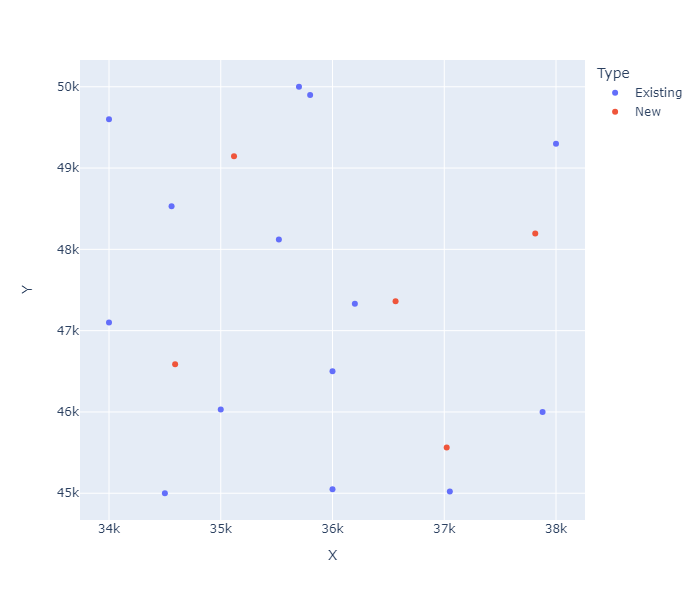
\includegraphics[width=0.5\textwidth]{figures/task4/task4-3.png}
          \caption{新井位置优化结果}
          \label{fig:NewWellsAndOldWells}
        \end{figure}
        首先,我们从新井的布局开始。如图 \ref{fig:NewWellsAndOldWells} 所示,新井(红色点)与现有井(蓝色点)的布局展示了新井的选址策略不仅考虑了资源量的最大化,同时也确保了合理的空间分布,避免过于集中或偏远。


  \item \textbf{资源量和不确定性分析}

        \begin{figure}[H]
          \centering
          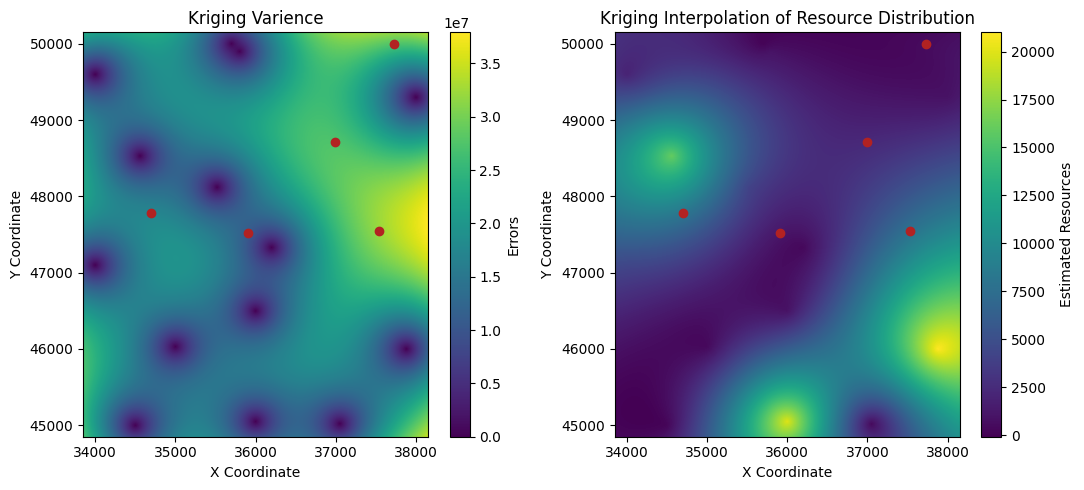
\includegraphics[width=0.8\textwidth]{figures/task4/task4-4.png}
          \caption{新井位置资源量情况}
          \label{fig:NewWellsAndResource}
        \end{figure}
        接下来,我们通过Kriging插值的结果来分析资源量分布和不确定性。如图 \ref{fig:NewWellsAndResource} 右侧所示,Kriging插值的资源分布图显示了预测的资源量,其中颜色越暗表示资源量越高。这帮助我们验证新井位置的选择是否位于资源丰富的区域。左侧的Kriging方差图表则提供了关于预测不确定性的信息,颜色越亮表示不确定性越高,这通常出现在样本点较少的区域。


  \item \textbf{井点距离的离散程度分析}
        \begin{figure}[H]
          \centering
          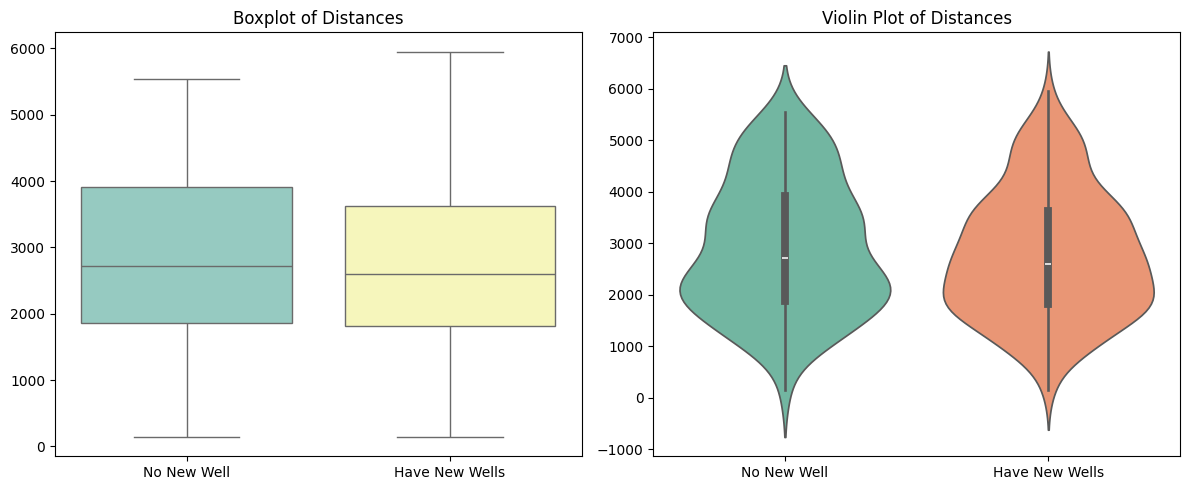
\includegraphics[width=0.8\textwidth]{figures/task4/task4-5.png}
          \caption{添加新井前后,所有井距离的离散程度}
          \label{fig:NewWellsAndNoNewWells}
        \end{figure}

        最后,我们分析了添加新井前后所有井点距离的离散程度。如图 \ref{fig:NewWellsAndNoNewWells} 所示,通过箱型图和小提琴图可以看出,引入新井后,井点之间的距离的中位数有所降低,这表明新井的加入使得井点分布更加均匀。小提琴图进一步揭示了数据分布的密度和范围,展示了新井引入前后井点距离分布的变化。

\end{enumerate}


\section{模型的评价与推广}

\subsection{模型的评价}
\subsubsection{模型的优点}
\begin{enumerate}
  \item \textbf{简洁性与计算效率:}本模型采用简便且成熟的方法论,通过简化的概率函数进行表达,有效减少计算量。此外,模型构建基于一系列合理的假设,例如,假设观测期内储层参数稳定,这对于保持数据在水平维度上的研究价值至关重要。此外,假设研究区域内的地质结构相对均质,并排除具有天然气特性的干扰物质,为模型提供了良好的环境条件。
  \item \textbf{数据预处理与质量控制:}在模型建立之前,进行了广泛的数据预处理工作,包括数据格式的标准化和异常值的剔除,这些步骤显著提高了数据的纯净度和准确性,从而增强了模型的准确性和可靠性,确保了结果的合理性,减少了数据本身可能引入的误差。
  \item \textbf{明确的建模目标:}模型针对天然气水合物资源量进行估计,明确界定了资源分布范围、资源参数的概率分布及其变化规律、资源量的概率分布估计以及增钻井位策略等关键问题,使得研究目标具体化且清晰。
  \item \textbf{综合多种数学模型:}本研究结合了多种数学模型,包括高斯混合模型(GMM)、正态分布拟合、核密度估计(KDE)和克里金插值(Kriging)。这些模型从不同的角度分析数据,增加了结果的全面性和深度。
\end{enumerate}

\subsubsection{模型的缺点}
\begin{enumerate}
  \item \textbf{模型与现实的假设差异:}尽管本研究基于地壳稳定性和参数均一性等关键假设建立模型,但现实中的地质情况远比模型所能涵盖的更为复杂。因此,模型在特定条件下理论上是合理的,但可能无法始终准确预测所有现实世界条件下的地质现象,存在一定的主观性。
  \item \textbf{模型参数的局限性:}由于研究条件和指导的限制,模型在构建时未能包含所有可能影响结果的参数。模型中的参数缺乏全面的自相关性和共线性分析,这可能影响模型的预测能力。未来研究可以通过引入更广泛的参数集和更详尽的分析来弥补这一点。
  \item \textbf{误差分析与数据量限制:}模型的预测精度受限于可用数据量,导致较大的误差。尽管进行了数据预处理,但仍可进一步精细化以确保潜在误差的最小化。
\end{enumerate}



\subsection{模型的推广}
本文中采用的体积法模型在天然气水合物资源评估中表现出一定的效率和实用性,尤其适用于具有相对均一地质特征和充分数据支持的区域。然而,为了增强模型的广泛适用性和准确度,以下提出一些可能的推广和优化方向,这些方向虽然需要进一步研究和验证,但具有较高的创新潜力和实用价值。
\begin{enumerate}
  \item 集成动态地质过程模拟:尽管体积法提供了一个静态的资源评估框架,但真实的地质过程是动态的,包括温度、压力的变化以及相关的地质活动。可以考虑开发一种集成模型,该模型能够模拟和预测这些动态过程对天然气水合物稳定性和可开采性的影响。通过引入时间维度,模型不仅能估算当前的资源量,还能预测资源的未来可利用性。
  \item 引入空间统计和地统计学方法:为了更精确地处理地质参数的空间变异性,模型可以集成先进的空间统计和地统计学方法,如变异函数分析和多点统计模拟。这些方法可以更好地描述和模拟地质参数的空间相关性和不确定性,提高资源量估算的空间精度。
  \item 经济因素的集成分析:在资源评估模型中引入经济学参数,如开采成本、市场价格和技术进步,可以构建一个更加综合的评估模型。这种经济-地质集成模型不仅可以预测资源量,还可以提供资源开发的经济可行性分析,为决策者提供更全面的决策支持。
  \item  多尺度模型开发:开发一个多尺度模型,可以同时处理区域尺度和局部尺度的地质数据。这种模型能够综合考虑大范围的地质结构特征与小范围的地质细节,提供更为精细化的资源评估。
  \item  可持续性评估的集成:在模型中加入环境影响评估模块,可以预测资源开发对环境的潜在影响,如温室气体排放、生态干扰等。这种集成可以帮助制定更为可持续的资源开发策略,符合全球可持续发展的要求。
\end{enumerate}
为了确保模型的准确性不受损害,我们舍弃了数据集里面的大量异常点,以提高数据质量,以避免任何可能的偏差对分析结果造成不利影响。尽管这一做法无可避免地导致了信息的损失,但它是确保研究严谨性的必要步骤,我们对于无法将它们纳入最终模型表示遗憾。如果不受时间限制的约束,我们可以投入更多的时间和资源,对全部数据点进行深入分析和处理。这将使我们能够构建一个更为全面和精确的模型,从而更准确地反映数据的真实分布和内在关系。

\section{模型的改进}
\subsection{成藏思路模型的改进}
当前成藏模型主要基于静态赋存特征,而实际的天然气水合物赋存状态受多种动态地质过程影响。天然气水合物的形成和稳定主要发生在高压环境中,当地层压力降低,例如由于构造运动导致的地层抬升或侵蚀,水合物可能会分解释放出甲烷气体。
天然气水合物在低温条件下更稳定,深海或冻土环境中有助于维持水合物的结构,因为温度较低。假如水底地热活动或全球变暖导致的海底温度上升,可能导致水合物不稳定并分解。
水流的侵蚀作用可能破坏水合物结构,导致其分解。
因此我们可以考虑更多的地质因素,如地层压力、温度变化、流体运动等,因为这些都可能影响天然气水合物的稳定性和分布。

\subsection{Kriging插值的改进}
Kriging 插值是一种高级的地统计学方法,用于预测空间数据的分布。在本研究中,我们使用普通 Kriging 模型(Ordinary Kriging)来估计未
知位置的资源量,基于已知井点的资源数据。
变异函数在描述点与点位置中起到了非常关键的左右,球状、指数和高斯模型是最常见最方便的模型,我们选择了球状变异函数模型,但可能并不是最适合的模型。
模型泛化方面,Kriging模型在样本点密集区域表现良好,在样本稀疏区域能力不足。我们的外部信息有限,无法过多引入从而提高泛化能力。

\subsection{粒子群算法的改进}
粒子群优化算法是一种基于群体智能的优化算法,它通过模拟鸟群或鱼群的社会行为来搜索最优解。
粒子群优化算法中的惯性权重控制着粒子的探索和开发平衡,固定的惯性权重可能导致早熟收敛或探索不足,而我们为了计算简便,将权重设置为了固定值0.7。
可能的优化包括自适应调整惯性权重,比如从较大的值开始逐渐减小,以及学习因子的动态调整,虽然不是必要操作但可以提高模型性能。
如果可能,粒子群优化算法与其他优化算法(如遗传算法、模拟退火)杂交,或许会有更好的效果。


\newpage

\nocite{*}
\printbibliography

\newpage
\begin{appendices}
  \section*{纯 Python 代码部分}

  \textbf{\textcolor[rgb]{0.98,0.00,0.00}{程序一:加载数据和预处理}}
  \lstinputlisting[language=python]{code/loadAndPreprocess.py}
  \textbf{\textcolor[rgb]{0.98,0.00,0.00}{程序二:拟合三维 Kriging 插值模型}}
  \lstinputlisting[language=python]{code/kriging3D-train.py}
  \textbf{\textcolor[rgb]{0.98,0.00,0.00}{程序三:使用三维 Kriging 模型进行预测}}
  \lstinputlisting[language=python]{code/kriging3D-predict.py}

  \section*{Jupyter Note Book(Plotly 输出不可读)}
  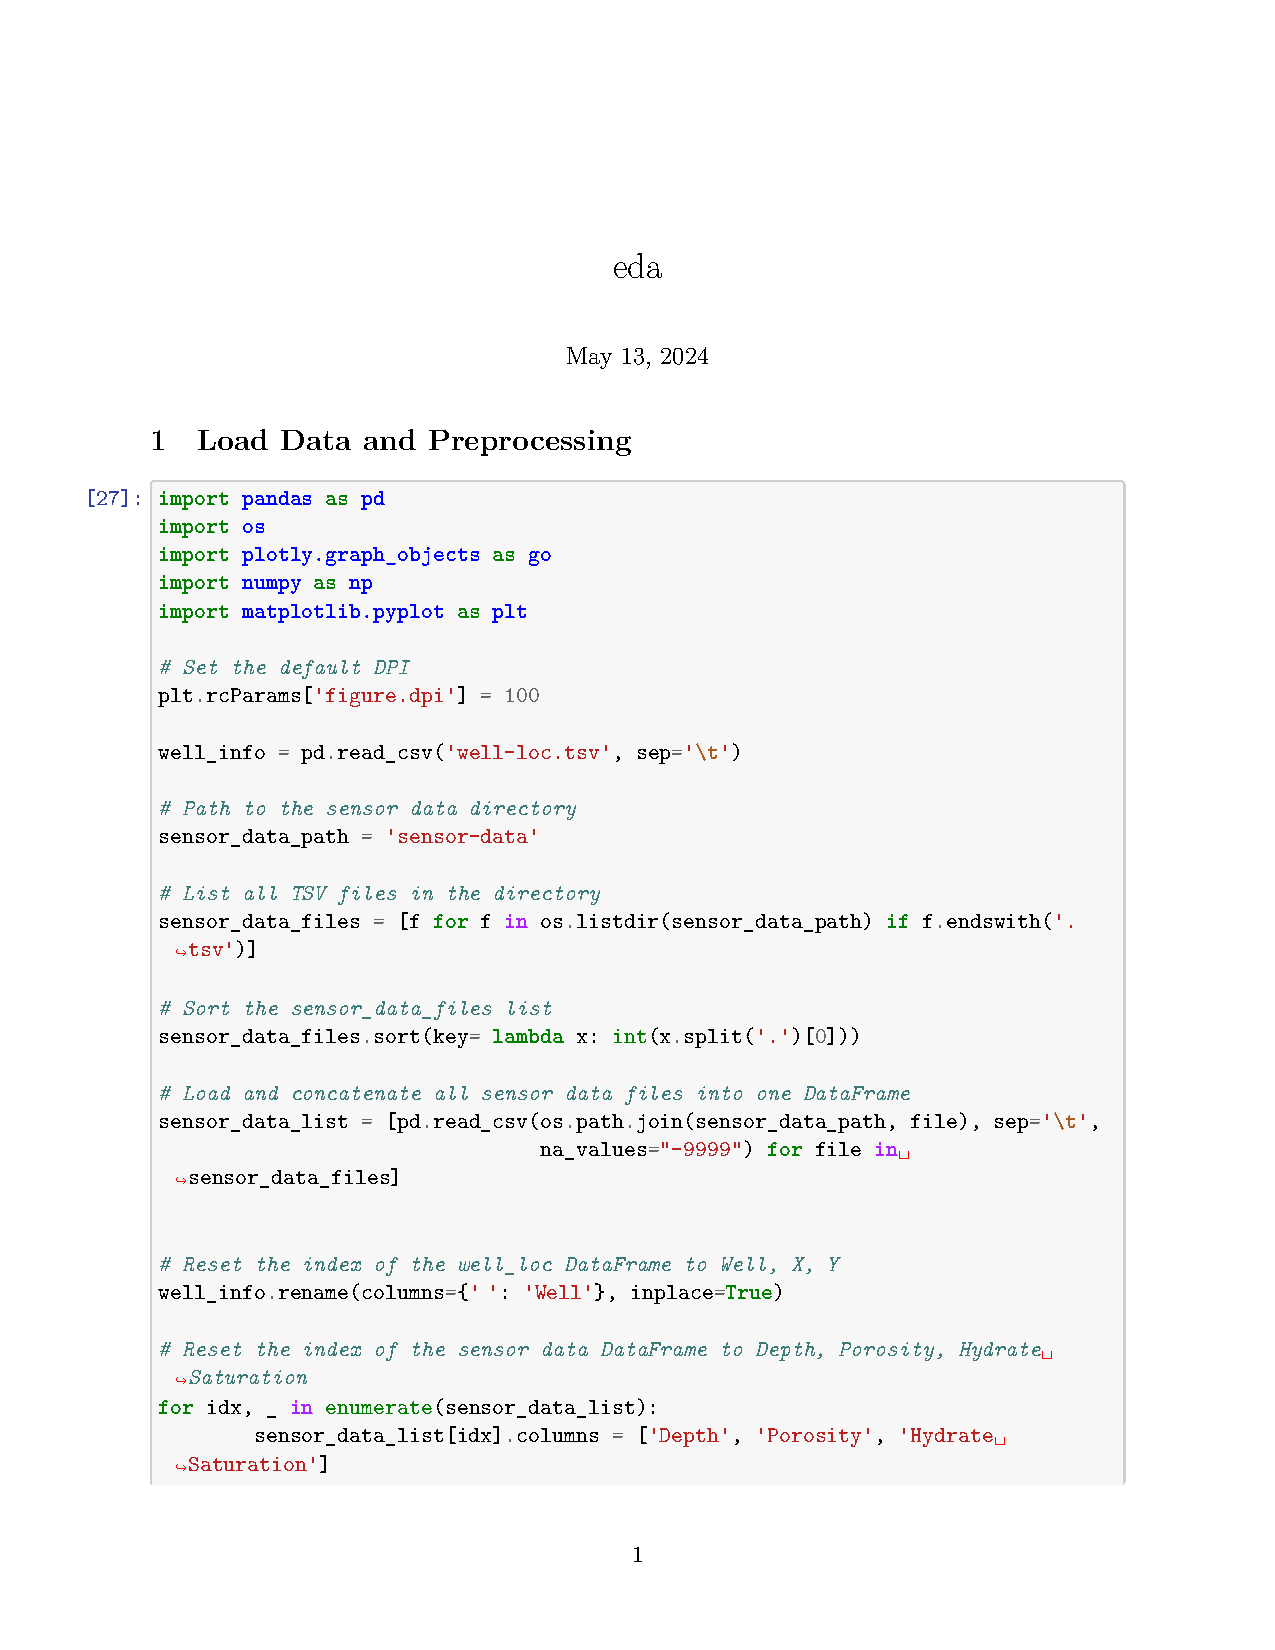
\includepdf[pages=-, scale=0.8, pagecommand={}]{code/jupyter/eda.pdf}
  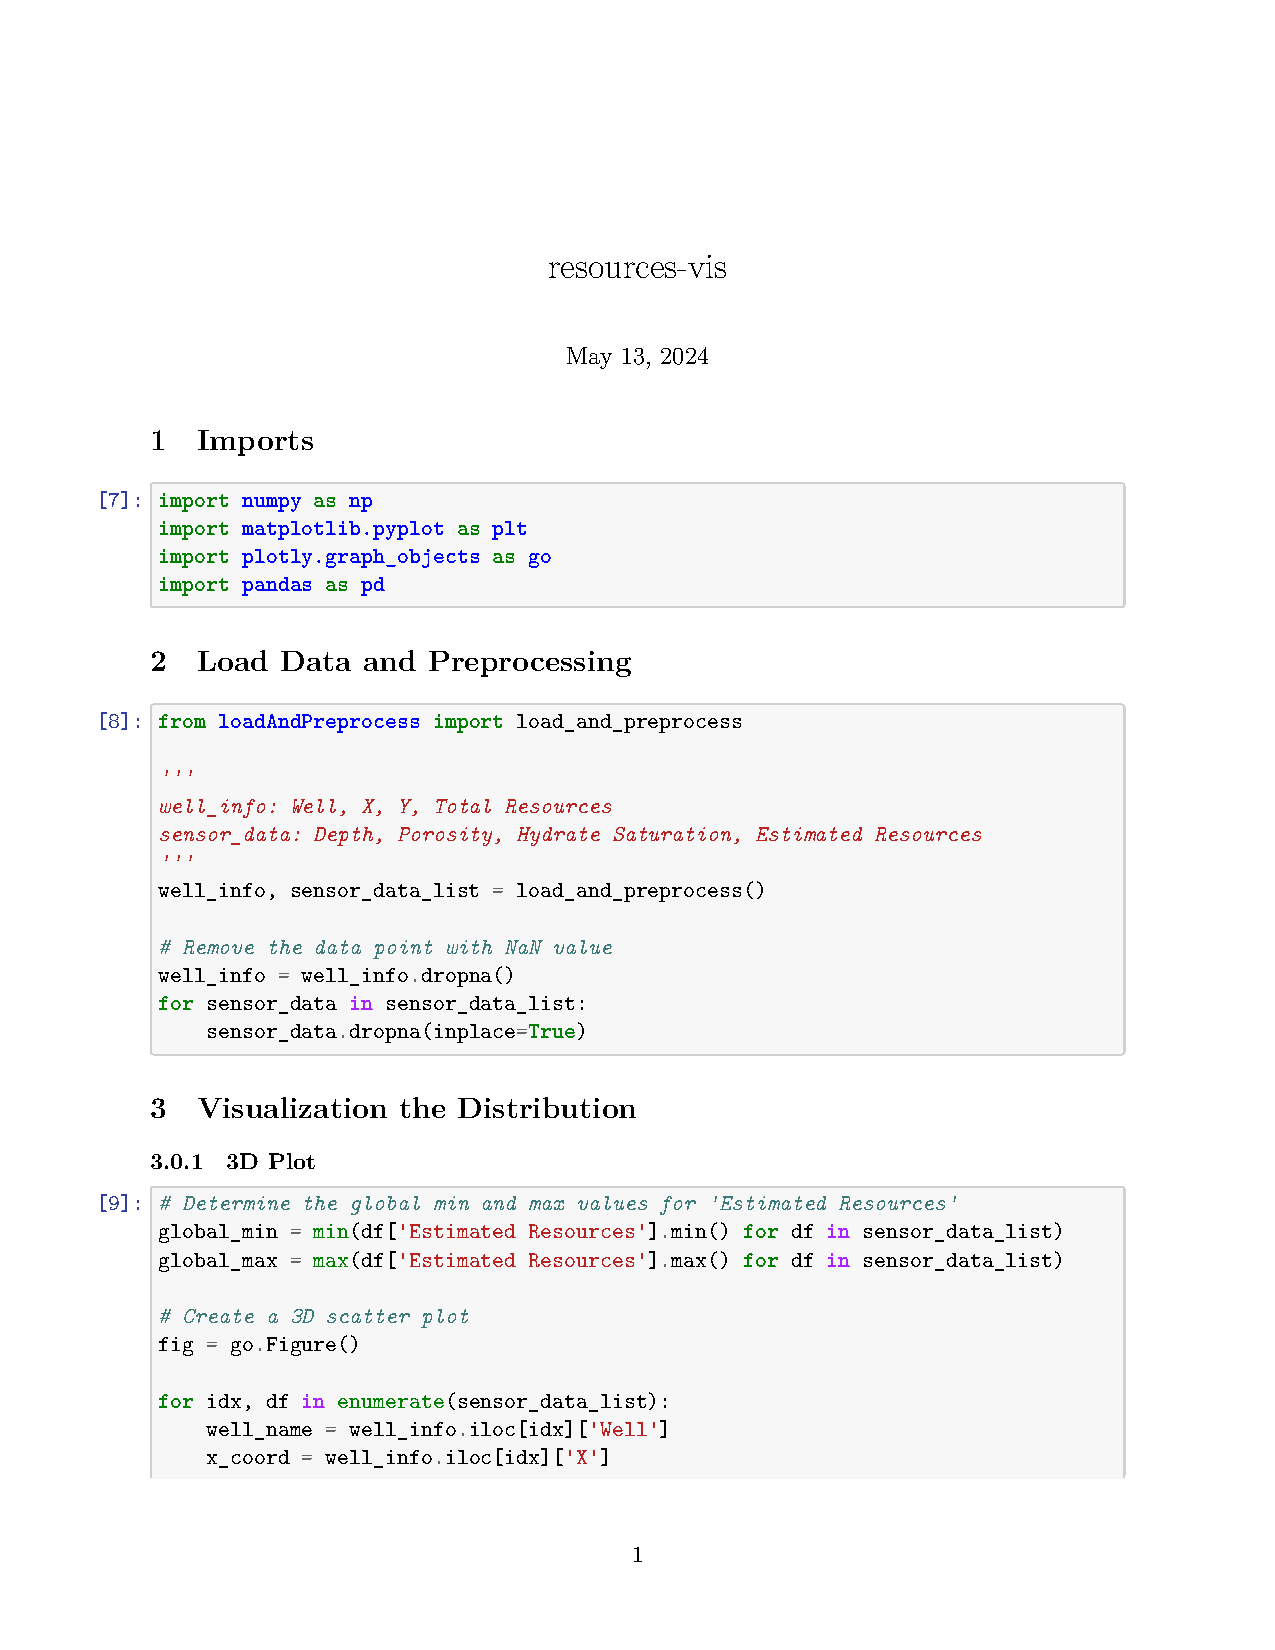
\includepdf[pages=-, scale=0.8, pagecommand={}]{code/jupyter/resources-vis.pdf}
  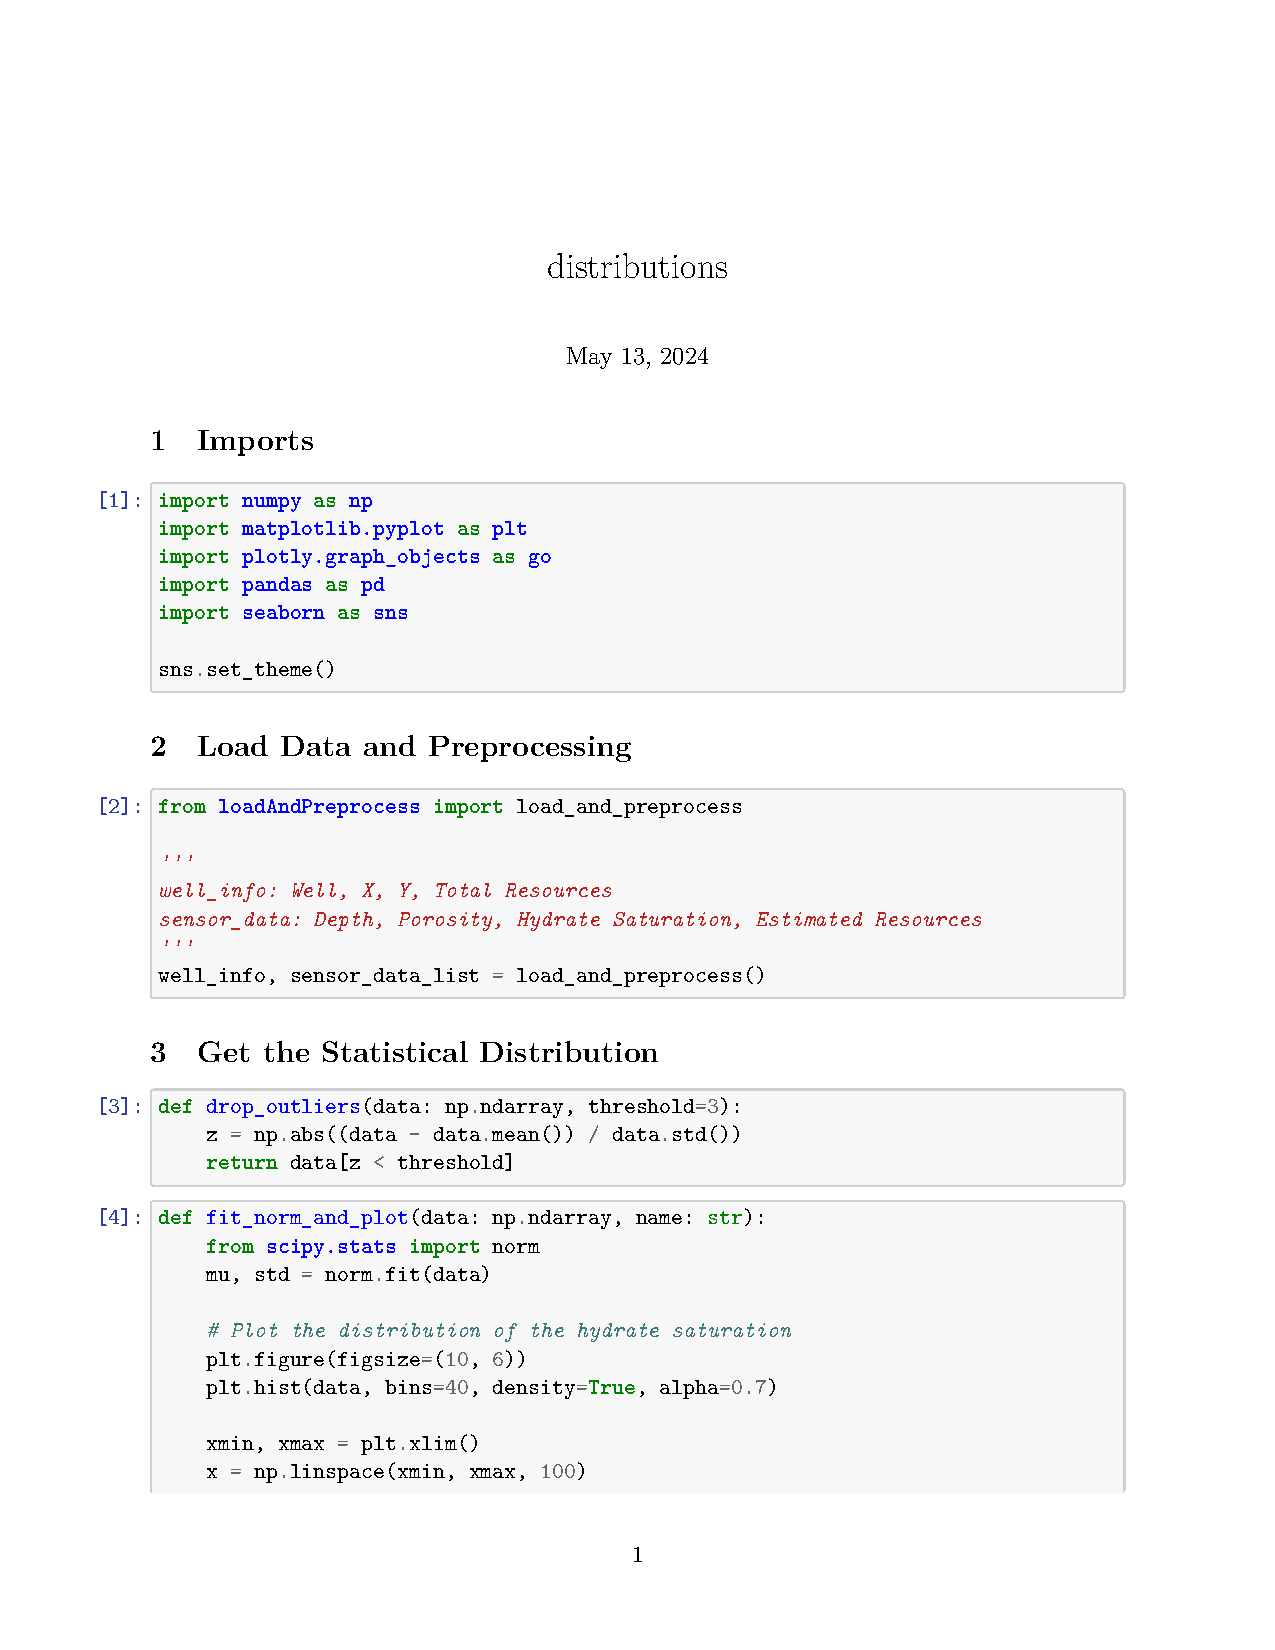
\includepdf[pages=-, scale=0.8, pagecommand={}]{code/jupyter/distributions.pdf}
  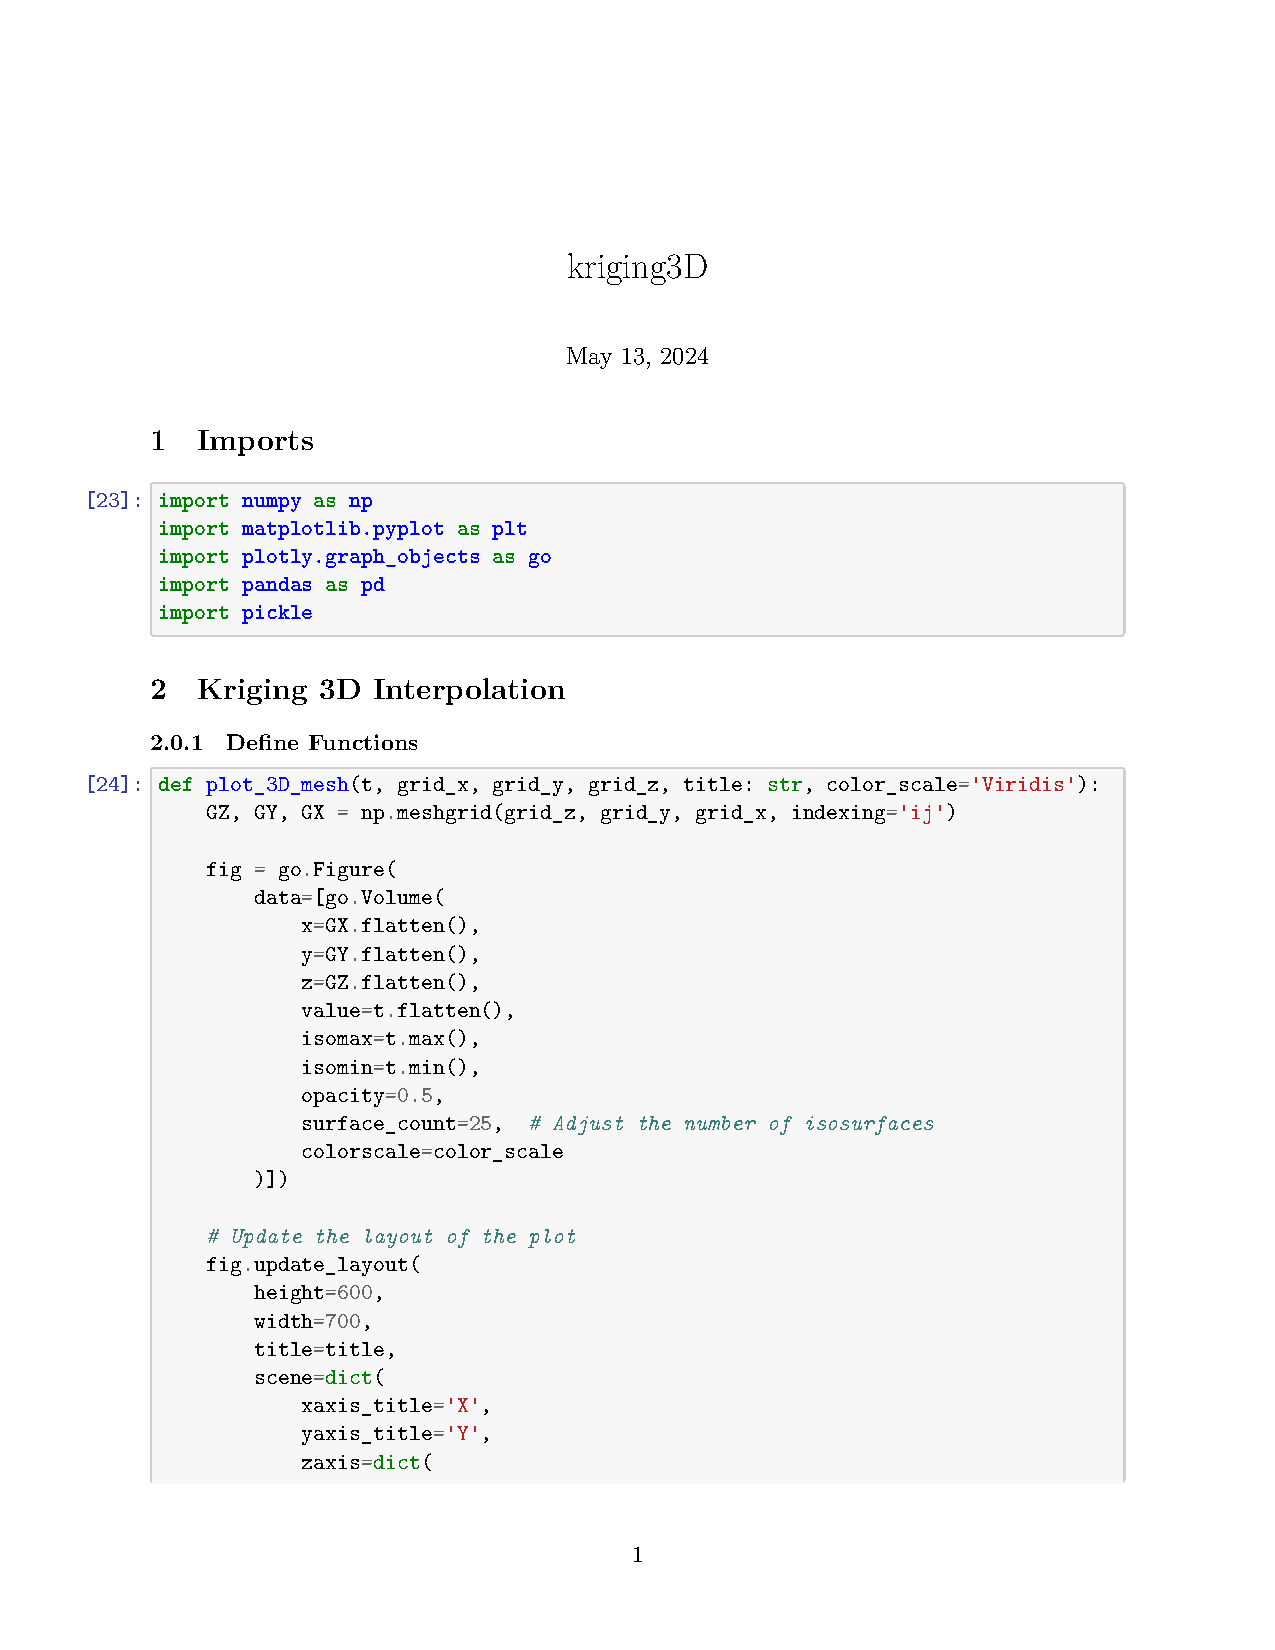
\includepdf[pages=-, scale=0.8, pagecommand={}]{code/jupyter/kriging3D/kriging3D.pdf}
  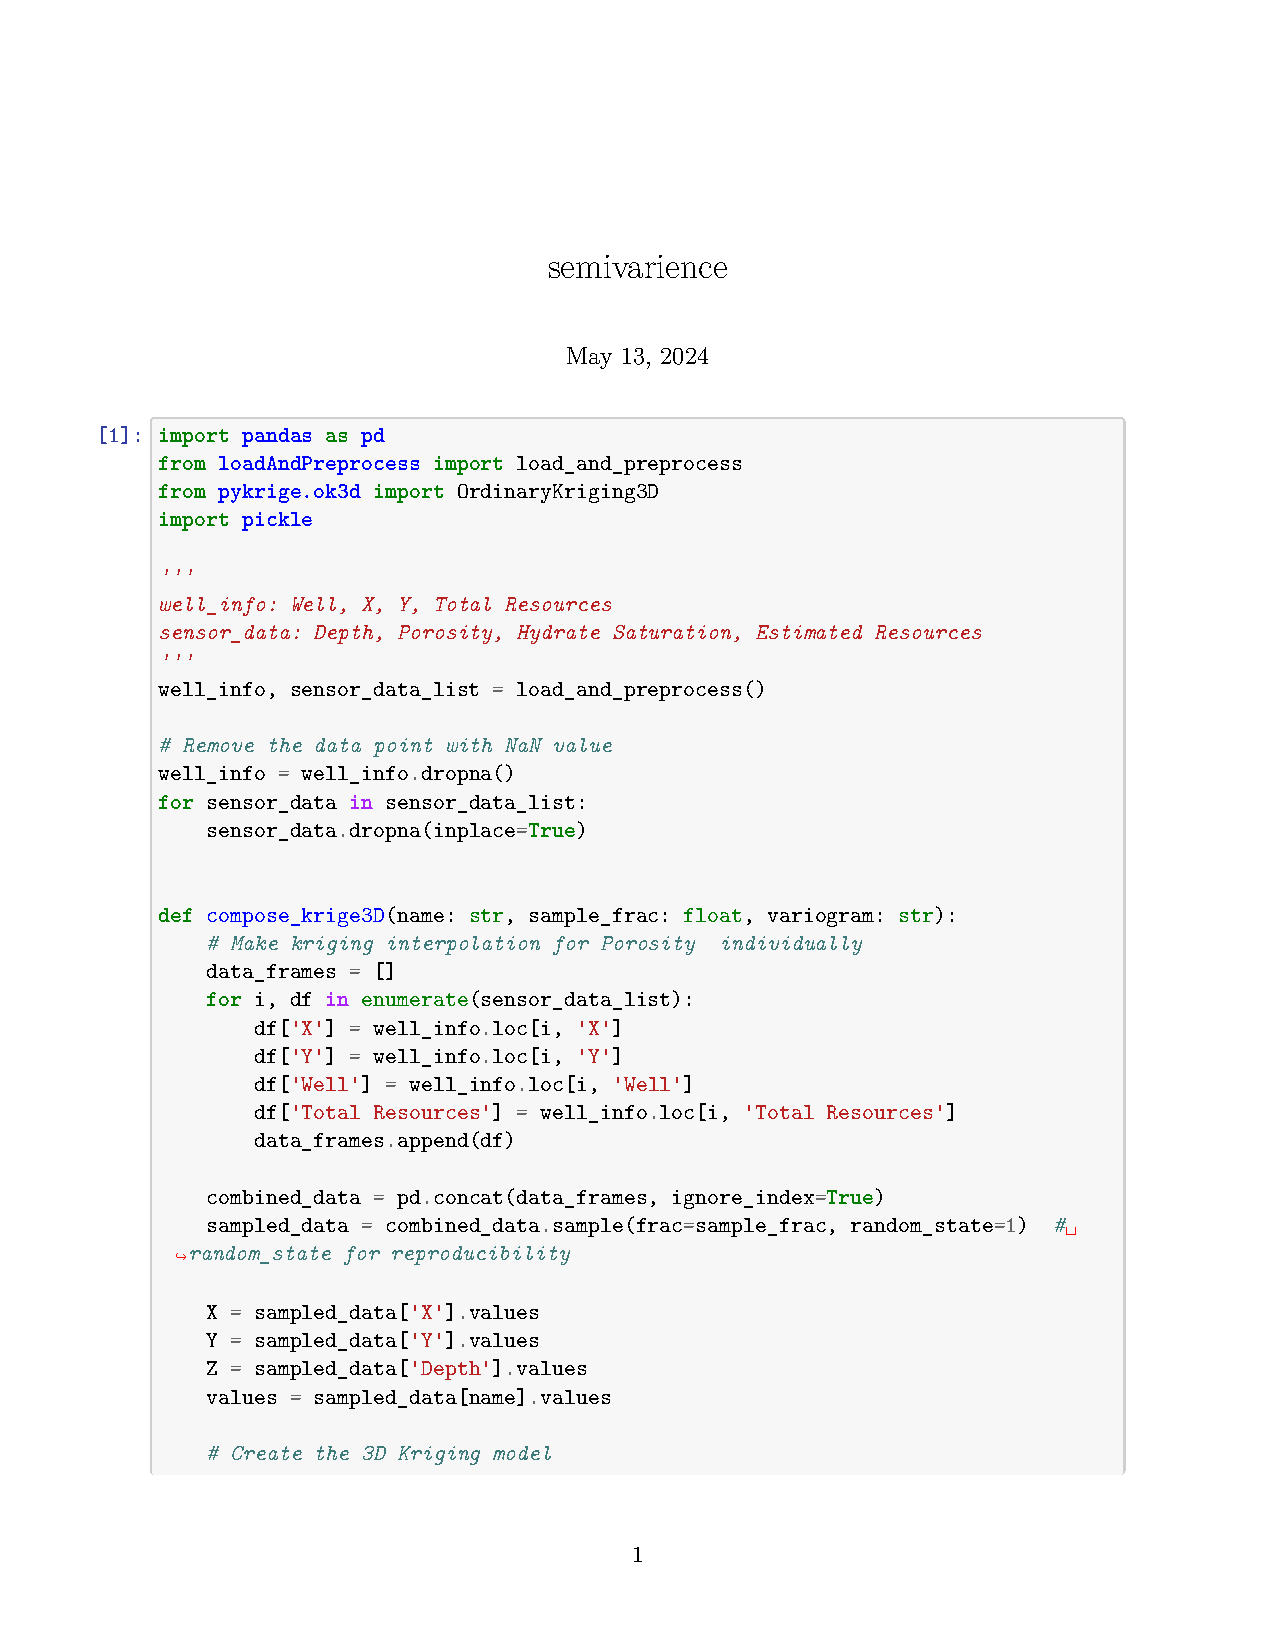
\includepdf[pages=-, scale=0.8, pagecommand={}]{code/jupyter/kriging3D/semivarience.pdf}
  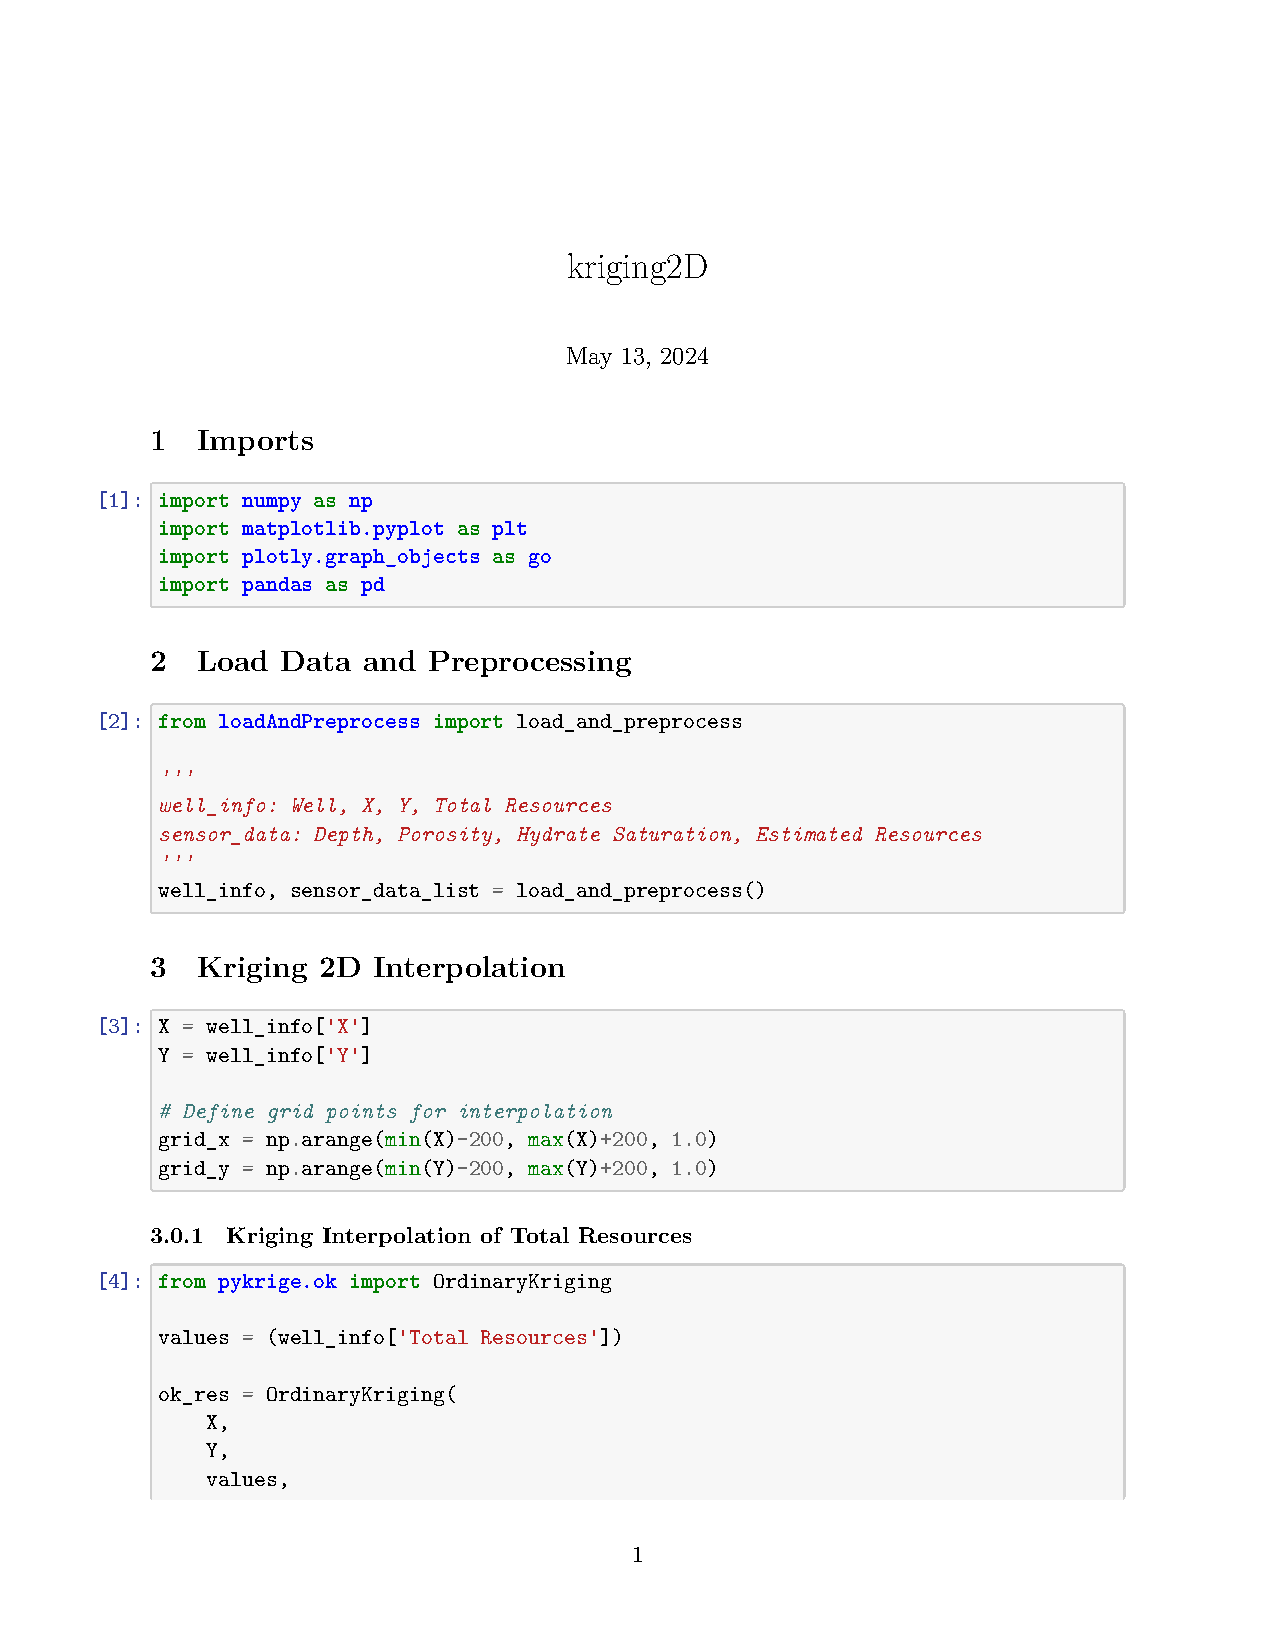
\includepdf[pages=-, scale=0.8, pagecommand={}]{code/jupyter/kriging2D.pdf}
  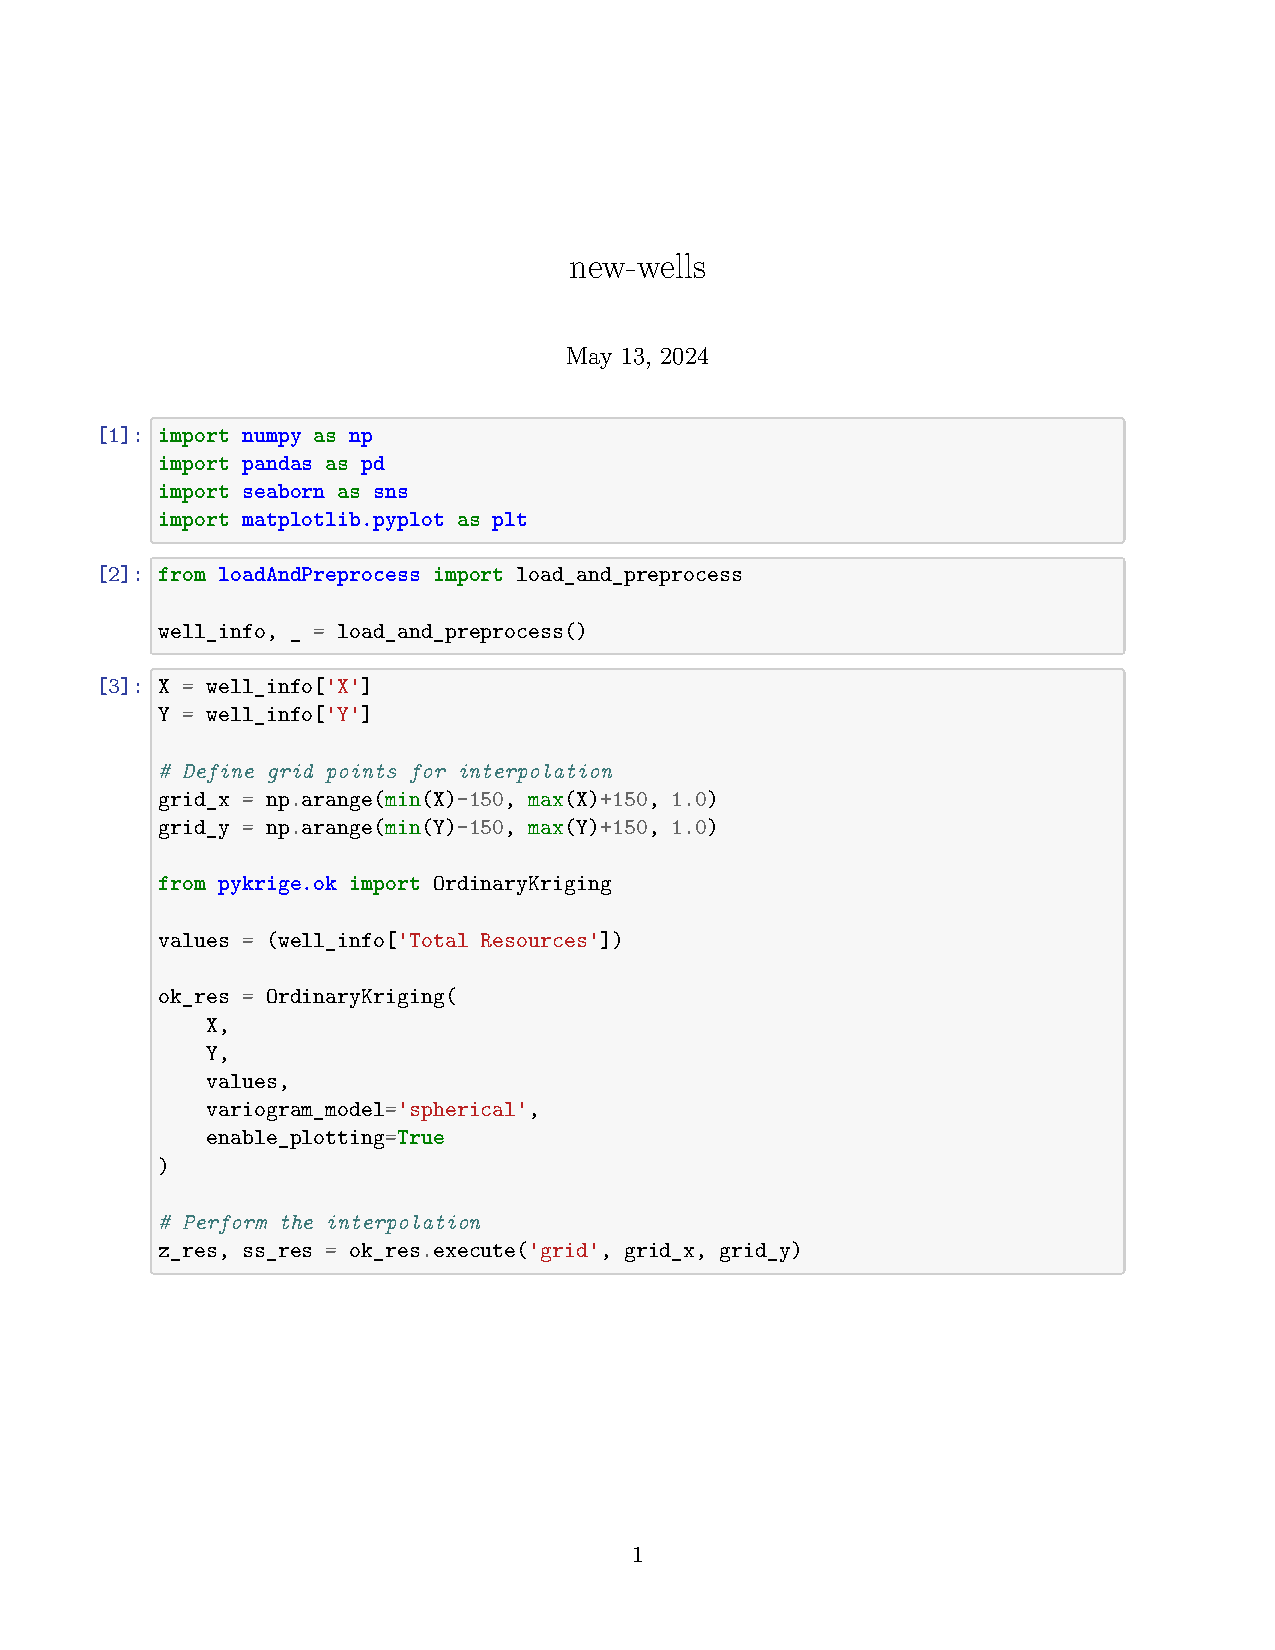
\includepdf[pages=-, scale=0.8, pagecommand={}]{code/jupyter/new-wells.pdf}
\end{appendices}
\end{document}
%%
%% This work consists of these files mcmthesis.dtx,
%%                                   figures/ and
%%                                   code/,
%% and the derived files             mcmthesis.cls,
%%                                   mcmthesis-demo.tex,
%%                                   README,
%%                                   LICENSE,
%%                                   mcmthesis.pdf and
%%                                   mcmthesis-demo.pdf.
%%
%% End of file `mcmthesis-demo.tex'.
